\chapter{Appendix}  \label{chap:Appendix}

All the supplementary material can be found on the attached USB-Stick and with exception of the FASTA file in the GitHub repository\footnote{\url{https://github.com/ahenoch/Masterthesis.git}}. The FASTA can be found FSU-Cloud\footnote{\url{https://cloud.uni-jena.de/s/fYkQ2NAwjND8oEM}}.

\begin{tabbing}
    \hspace{4cm}\=\=\kill
    \texttt{Graphics/} \> Folder containing all graphics created with \texttt{Inkscape}\\
    \texttt{PCA/} \> Folder containing all PK and PD method comparison results\\
    \texttt{Results/} \> Folder containing the result of every segments final clustering\\
    \texttt{Thesis/} \> Folder containing the components of written the thesis\\
    \texttt{UMAP/} \> Folder containing all UK and UD method comparison results\\
    \texttt{A.fasta} \> The FASTA file used in the project\\
    \texttt{Clustering.py} \> The \textit{Influenza A Virus} clustering tool\\
    \texttt{Environment.yml} \> The configuration file for recreation of the used environment\\
    \texttt{PCA.ipynb} \> The pipeline used for the PK and PD method comparison\\
    \texttt{README.md} \> The instructions for usage of the clustering tool\\
    \texttt{Thesis.pdf} \> The written thesis\\
    \texttt{UMAP.ipynb} \> The pipeline used for the UK and UD method comparison\\
\end{tabbing}

Supplementary tables and graphics directly linked in the thesis can be found on the following pages.

% \begin{table}[!hbt]
%     \centering
%     \caption[Cluster database with PK]{\textbf{Cluster database with PK.}.}
%     \label{tab:PCA_Cluster_Database}
%     \pgfplotstabletypeset[
%         every head row/.style={
%             before row={
%                 \toprule
%             },
%             after row={
%                 \midrule
%             },
%         },
%         every last row/.style={
%             after row={
%                 ... & ... & ... & ... & ... & ... & ... \\
%                 \bottomrule
%             },
%         },
%         begin table=\begin{tabular*}{\textwidth},
%         end table=\end{tabular*},
%         columns={0,1,2,3,4,5,6},
%         columns/0/.style={string type,multicolumn names=l,column name=\textbf{Accession}, column type=@{\extracolsep{\fill}\hspace{6pt}}r},
%         columns/1/.style={int detect, multicolumn names=l,column name=\textbf{Segment}, column type=r},
%         columns/2/.style={int detect, multicolumn names=l,column name=\textbf{Cluster}, column type=r},
%         columns/3/.style={string type,multicolumn names=l,column name=\textbf{H}, column type=r},
%         columns/4/.style={string type,multicolumn names=l,column name=\textbf{Centroid}, column type=r},
%         columns/5/.style={string type,multicolumn names=l,column name=\textbf{N}, column type=r},
%         columns/6/.style={string type,multicolumn names=l,column name=\textbf{Strain}, column type=r},
%     ]
%     {PCA/cluster_head.csv}
% \end{table}

% \newpage

% \begin{table}[!hbt]
%     \centering
%     \caption[Cluster database with UK]{\textbf{Cluster database with UK.}.}
%     \label{tab:UMAP_Cluster_Database}
%     \pgfplotstabletypeset[
%         every head row/.style={
%             before row={
%                 \toprule
%             },
%             after row={
%                 \midrule
%             },
%         },
%         every last row/.style={
%             after row={
%                 ... & ... & ... & ... & ... & ... & ... \\
%                 \bottomrule
%             },
%         },
%         begin table=\begin{tabular*}{\textwidth},
%         end table=\end{tabular*},
%         columns={0,1,2,3,4,5,6},
%         columns/0/.style={string type,multicolumn names=l,column name=\textbf{Accession}, column type=@{\extracolsep{\fill}\hspace{6pt}}r},
%         columns/1/.style={int detect, multicolumn names=l,column name=\textbf{Segment}, column type=r},
%         columns/2/.style={int detect, multicolumn names=l,column name=\textbf{Cluster}, column type=r},
%         columns/3/.style={string type,multicolumn names=l,column name=\textbf{H}, column type=r},
%         columns/4/.style={string type,multicolumn names=l,column name=\textbf{Centroid}, column type=r},
%         columns/5/.style={string type,multicolumn names=l,column name=\textbf{N}, column type=r},
%         columns/6/.style={string type,multicolumn names=l,column name=\textbf{Strain}, column type=r},
%     ]
%     {UMAP/cluster_head.csv}
% \end{table}

\newpage

\begin{figure}[!htb]
    \centering
    %\begin{adjustbox}{minipage=\dimexpr\textwidth-2\fboxsep-2\fboxrule,fbox}
    \begin{subfigure}[b]{0.475\textwidth}
        \caption[DBCV exploration]{\textbf{DBCV exploration}}
        \label{subfig:PCA_Cluster_DBCV_Explo_4}            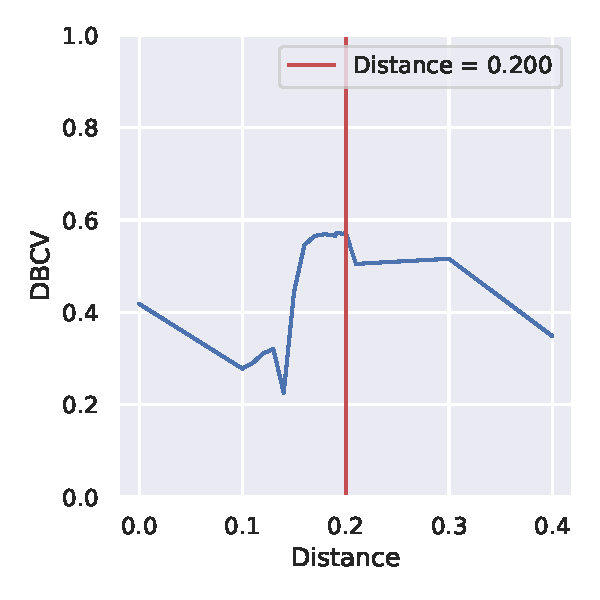
\includegraphics[width=\textwidth]{PCA/Cluster_DBCV_Segment_4.pdf}
    \end{subfigure}
    \hfill
    \begin{subfigure}[b]{0.475\textwidth}
        \caption[DBCV knee]{\textbf{DBCV knee}}
        \label{subfig:PCA_Cluster_DBCV_Elbow_4}            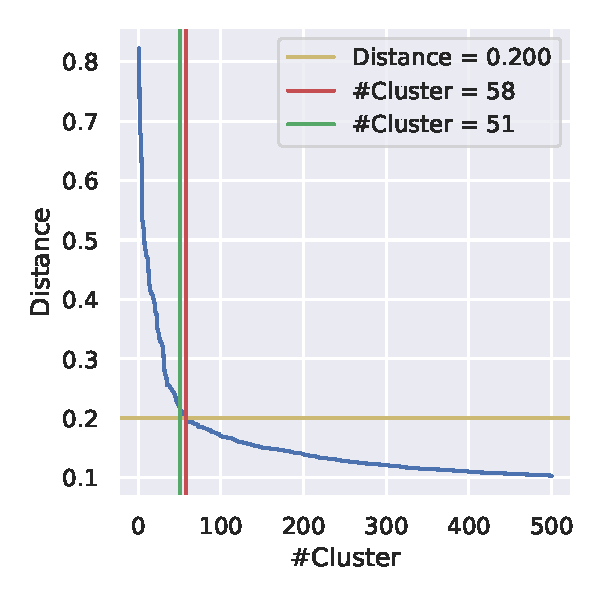
\includegraphics[width=\textwidth]{PCA/Cluster_Elbow_DBCV_Segment_4.pdf}
    \end{subfigure}
    \vskip\baselineskip
    \begin{subfigure}[b]{0.475\textwidth}
        \caption[Cluster distribution]{\textbf{Cluster distribution}}
        \label{subfig:PCA_Cluster_DBCV_Distribution_4}            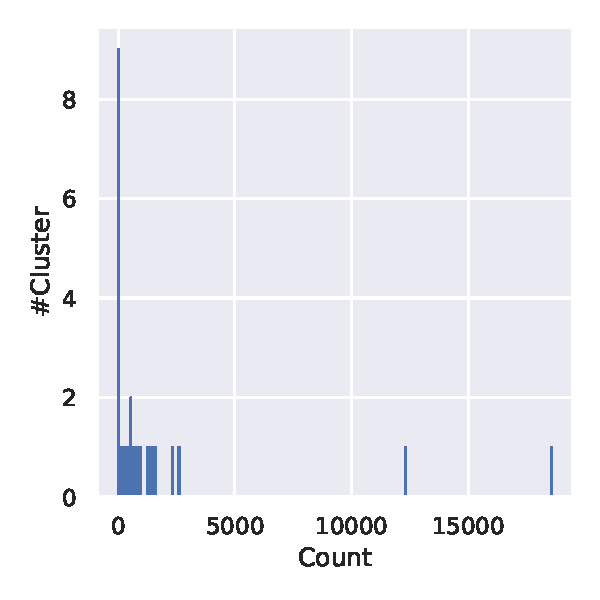
\includegraphics[width=\textwidth]{PCA/Cluster_Distribution_Segment_4_alternative.pdf}
    \end{subfigure}
    \hfill
    \begin{subfigure}[b]{0.475\textwidth}
        \caption[Logarithmic distribution]{\textbf{Logarithmic distribution}}
        \label{subfig:PCA_Cluster_DBCV_Distribution_log_4}            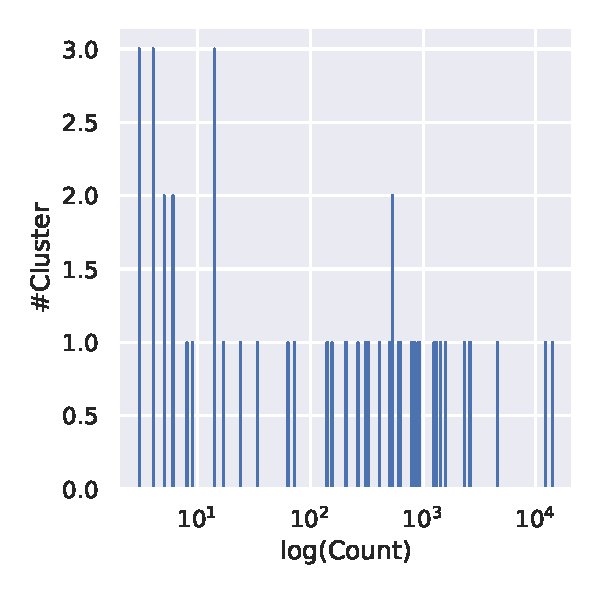
\includegraphics[width=\textwidth]{PCA/Cluster_Distribution_Log_Segment_4_alternative.pdf}
    \end{subfigure}
    %\end{adjustbox}
    \caption[Clustering of segment 4 with PD]{\textbf{Clustering of segment 4 with PD.} Segment 4 clustering, using the combination of \texttt{PCA} and the \gls{DBCV} exploration (PD) results in the given figure. The blue line is the \gls{DBCV} value resulting from hybrid \texttt{HDBSCAN} clustering with a given distance value $\varepsilon$. The highest \gls{DBCV} value and, therefore,resulting $\varepsilon$ value is described with the red line. The top right sub figure shows the absolute relation of the distance in the single linkage tree to the total number of clusters as the blue line. With the red line, the number of raw clusters, prior to the \texttt{HDBSCAN} part of the hybrid clustering is marked and the final cluster number after it in green. The yellow line describes the threshold, extracted from the maximum \glspl{DBCV} distance threshold $\varepsilon$, used to perform the hybrid clustering and to get the final cluster number. The red line in the top left sub figure denotes, thus, the same value as the yellow line in the top right sub figure, the distance threshold $\varepsilon$ located by the \gls{DBCV} exploration. The bottom sub figures give information about the distribution of the clusters sizes in continuous and logarithmic scale.}
    \label{fig:PCA_Cluster_DBCV_4}
\end{figure}

\FloatBarrier
\newpage

\begin{figure}[!htb]
    \centering
    %\begin{adjustbox}{minipage=\dimexpr\textwidth-2\fboxsep-2\fboxrule,fbox}
    \begin{subfigure}[b]{0.475\textwidth}
        \caption[DBCV exploration]{\textbf{DBCV exploration}}
        \label{subfig:UMAP_Cluster_DBCV_Explo_4}            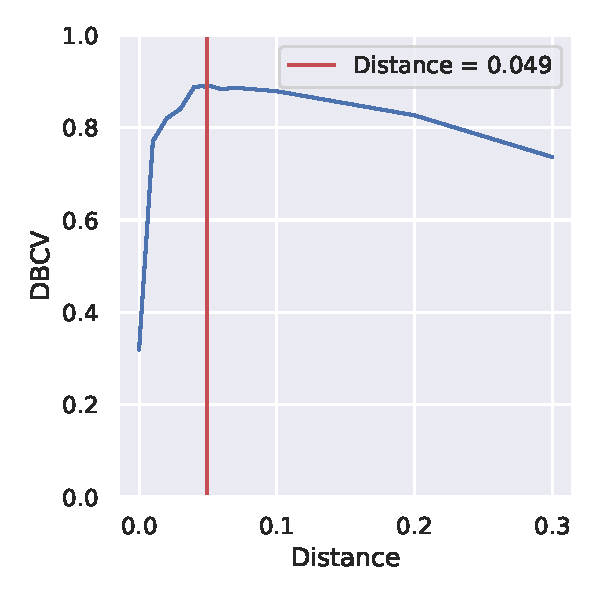
\includegraphics[width=\textwidth]{UMAP/Cluster_DBCV_Segment_4.pdf}
    \end{subfigure}
    \hfill
    \begin{subfigure}[b]{0.475\textwidth}
        \caption[DBCV knee]{\textbf{DBCV knee}}
        \label{subfig:UMAP_Cluster_DBCV_Elbow_4}            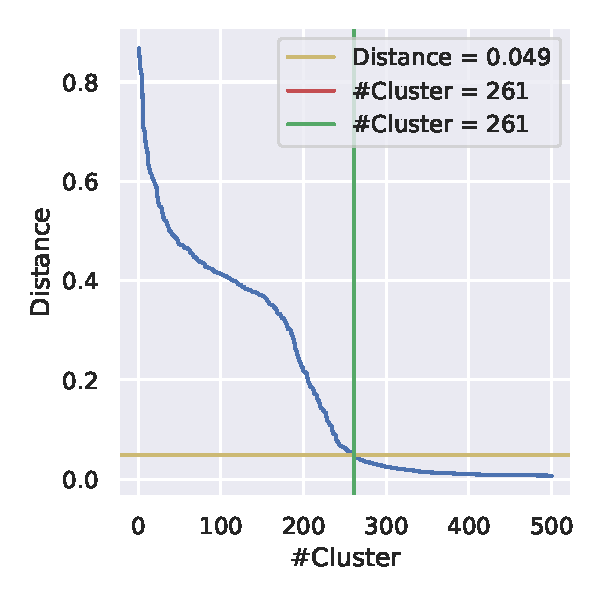
\includegraphics[width=\textwidth]{UMAP/Cluster_Elbow_DBCV_Segment_4.pdf}
    \end{subfigure}
    \vskip\baselineskip
    \begin{subfigure}[b]{0.475\textwidth}
        \caption[Cluster distribution]{\textbf{Cluster distribution}}
        \label{subfig:UMAP_Cluster_DBCV_Distribution_4}            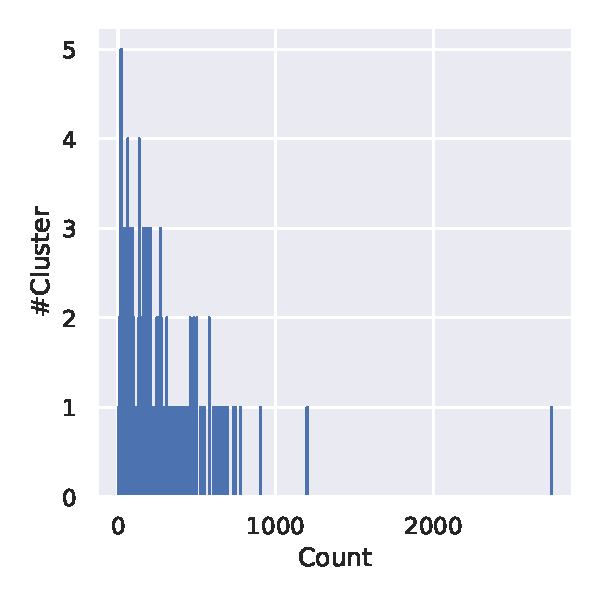
\includegraphics[width=\textwidth]{UMAP/Cluster_Distribution_Segment_4_alternative.pdf}
    \end{subfigure}
    \hfill
    \begin{subfigure}[b]{0.475\textwidth}
        \caption[Logarithmic distribution]{\textbf{Logarithmic distribution}}
        \label{subfig:UMAP_Cluster_DBCV_Distribution_log_4}            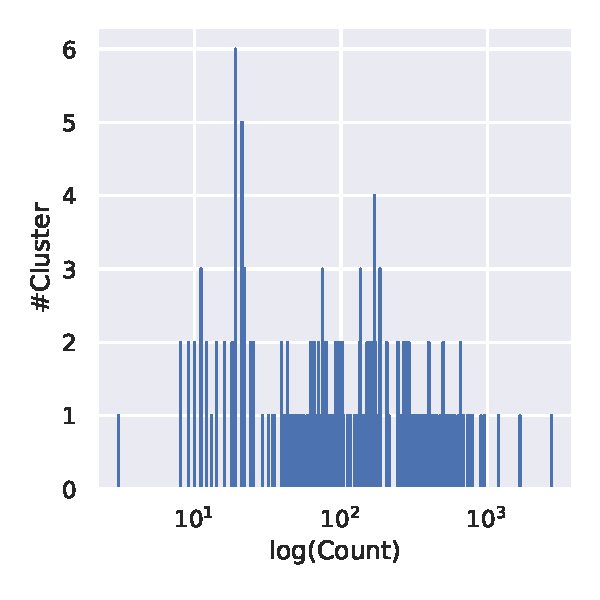
\includegraphics[width=\textwidth]{UMAP/Cluster_Distribution_Log_Segment_4_alternative.pdf}
    \end{subfigure}
    %\end{adjustbox}
    \caption[Clustering of segment 4 with UD]{\textbf{Clustering of segment 4 with UD.} Segment 4 clustering, using the combination of \texttt{PCA}, \texttt{UMAP} and the \gls{DBCV} exploration (UD) results in the given figure. The blue line is the \gls{DBCV} value resulting from hybrid \texttt{HDBSCAN} clustering with a given distance value $\varepsilon$. The highest \gls{DBCV} value and, therefore, resulting $\varepsilon$ value is described with the red line. The top right sub figure shows the absolute relation of the distance in the single linkage tree to the total number of clusters as the blue line. With the red line, the number of raw clusters, prior to the \texttt{HDBSCAN} part of the hybrid clustering is marked and the final cluster number after it in green. The yellow line describes the threshold, extracted from the maximum \glspl{DBCV} distance threshold $\varepsilon$, used to perform the hybrid clustering and to get the final cluster number. The red line in the top left sub figure denotes, thus, the same value as the yellow line in the top right sub figure,the distance threshold $\varepsilon$ located by the \gls{DBCV} exploration. The bottom sub figures give information about the distribution of the clusters sizes in continuous and logarithmic scale.}
    \label{fig:UMAP_Cluster_DBCV_4}
\end{figure}

\FloatBarrier
\newpage

\begin{figure}[!hbt]
    \centering
    %\begin{adjustbox}{minipage=\dimexpr\textwidth-2\fboxsep-2\fboxrule,fbox}
    \begin{subfigure}[b]{0.475\textwidth}
        \caption[Kneedle Algorithm]{\textbf{Kneedle Algorithm}}
        \label{subfig:UMAP_Cluster_Knee_Kneedle_4}            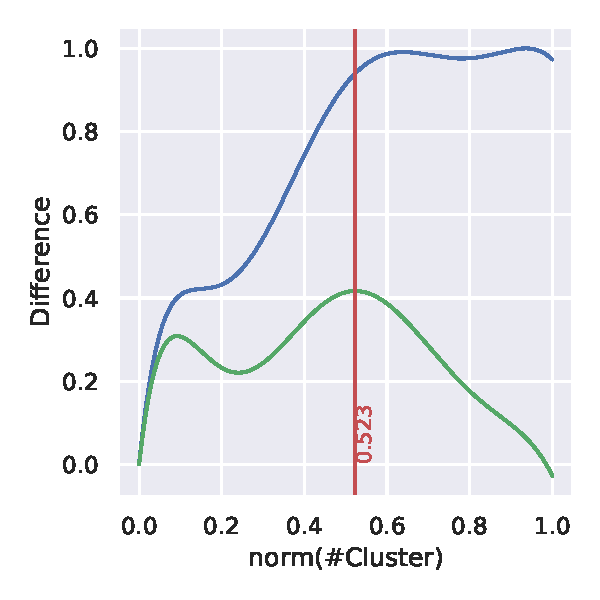
\includegraphics[width=\textwidth]{UMAP/Cluster_Knee_Segment_4.pdf}
    \end{subfigure}
    \hfill
    \begin{subfigure}[b]{0.475\textwidth}
        \caption[Knee Point]{\textbf{Knee Point}}
        \label{subfig:UMAP_Cluster_Knee_Elbow_4}            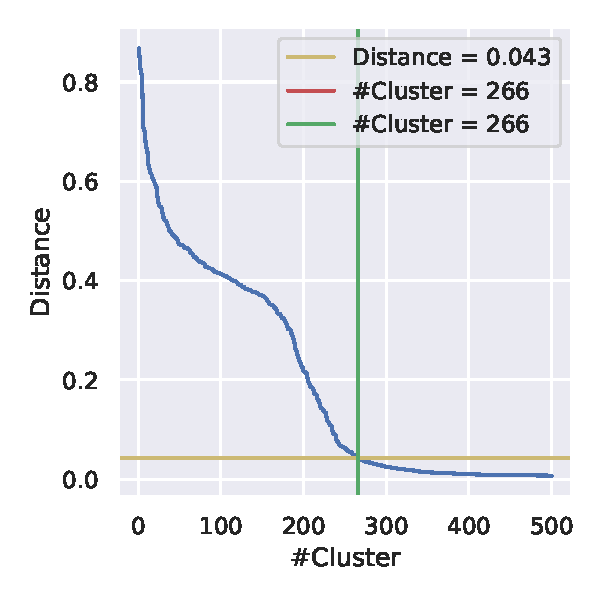
\includegraphics[width=\textwidth]{UMAP/Cluster_Elbow_Knee_Segment_4.pdf}
    \end{subfigure}
    \vskip\baselineskip
    \begin{subfigure}[b]{0.475\textwidth}
        \caption[Cluster distribution]{\textbf{Cluster distribution}}
        \label{subfig:UMAP_Cluster_Knee_Distributione_4}            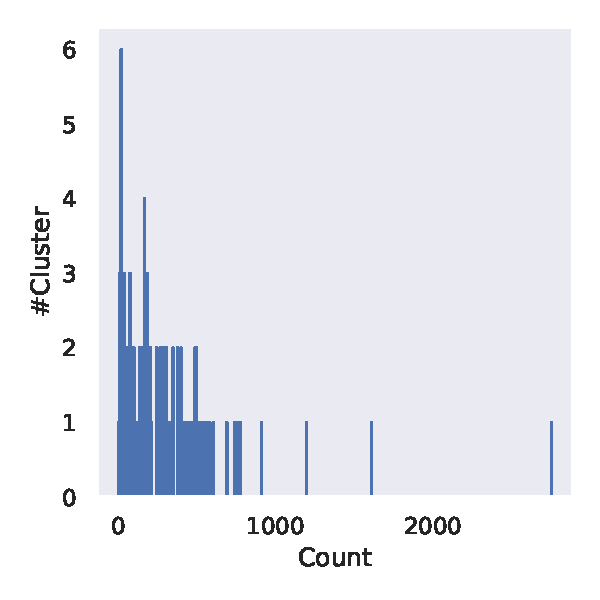
\includegraphics[width=\textwidth]{UMAP/Cluster_Distribution_Segment_4.pdf}
    \end{subfigure}
    \hfill
    \begin{subfigure}[b]{0.475\textwidth}
        \caption[Logarithmic distribution]{\textbf{Logarithmic distribution}}
        \label{subfig:UMAP_Cluster_Knee_Distribution_log_4}            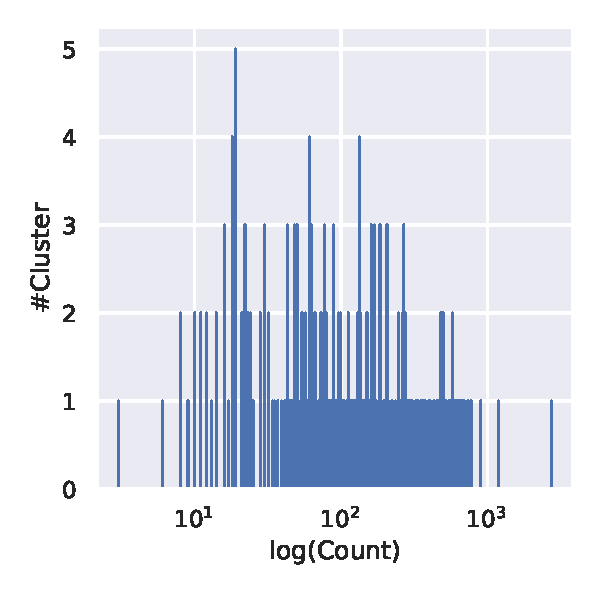
\includegraphics[width=\textwidth]{UMAP/Cluster_Distribution_Log_Segment_4.pdf}
    \end{subfigure}
    %\end{adjustbox}
    \caption[Clustering of segment 4 with UK]{\textbf{Clustering of segment 4 with UK.} Segment 4 clustering, using the combination of \texttt{PCA,} \texttt{UMAP} and the Kneedle Algorithm (UK) results in the given figure. The green curve in the top left sub figure describes the change of the distance in the single linkage tree with increasing normalized cluster number and, therefore, the location of the knee, as normalized cluster size at the maximum, highlighted by the red line. The blue line is the inverse polynomial representation of the blue line in top right subfigure. The top right sub figure shows the absolute relation of the distance in the single linkage tree to the total number of clusters as the blue line. With the red line, the number of raw clusters, prior to the \texttt{HDBSCAN} part of the hybrid clustering is marked and the final cluster number after it in green. The yellow line describes the threshold, extracted from the knees raw cluster number and, therefore, the $\varepsilon$ value used to perform the hybrid clustering and to get the final cluster number. The normalized cluster number in the red line in the top left sub figure is the raw cluster number in the top right sub figure calculated on the range of one to 500 clusters, thus, directly derived from it. The bottom sub figures give information about the distribution of the clusters sizes in continuous and logarithmic scale.}
    \label{fig:UMAP_Cluster_Knee_4}
\end{figure}

\FloatBarrier
\newpage

\begin{figure}[!hbt]
    \centering
    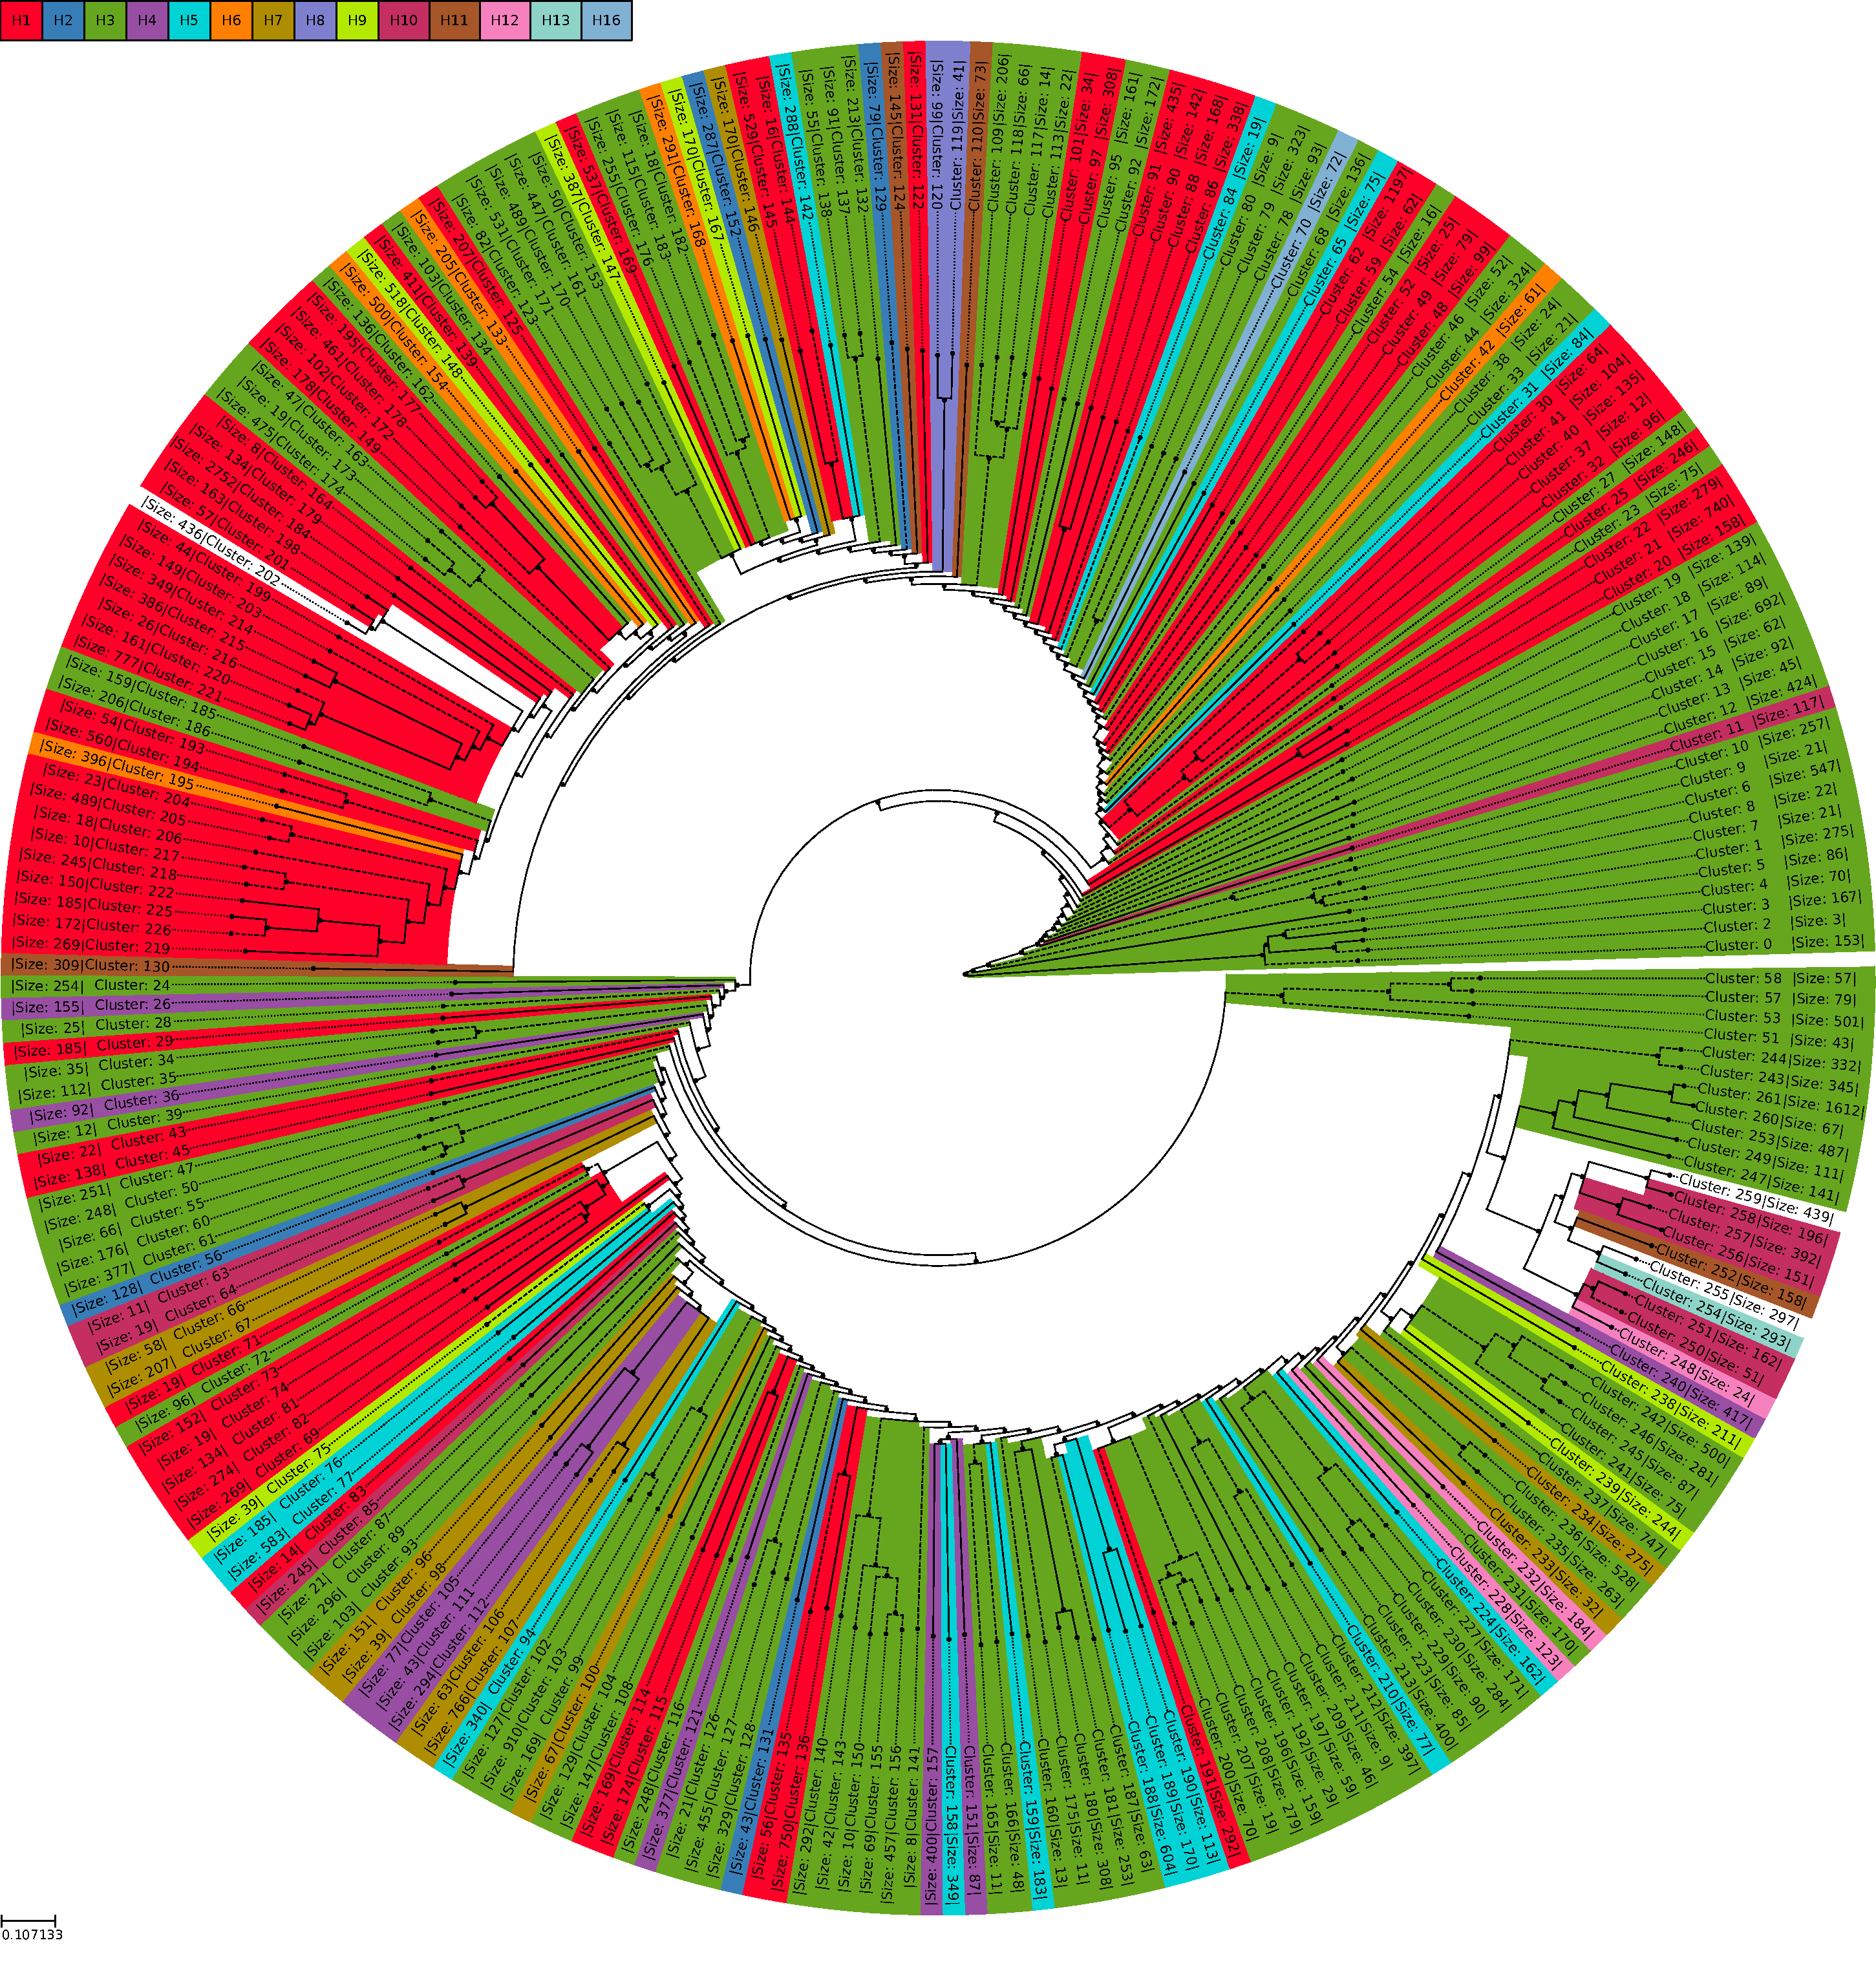
\includegraphics[width=\textwidth]{UMAP/Clustertree_Segment_4_H_Knee.pdf}
    \caption[Clustering tree of segment 4 with UK]{\textbf{Clustering tree of segment 4 with UK.} The cluster tree of segment 4 clustering, using the combination of \texttt{PCA}, \texttt{UMAP} and the Kneedle Algorithm (UK) (\autoref{fig:UMAP_Cluster_Knee_4}). The labeling of the clusters in the tree is based on the subtype of the contained sequences. Unclassified sequences of a cluster are reclassified as a given subtype if sequences of only this subtype are present in the cluster in addition to the unclassified ones. Unlabeled clusters contain sequences from at least two subtypes and zero or more unclassified sequences. Two clusters are mixed since containing sequences of more than one subtype (\autoref{tab:Cluster_Knee}).}
    \label{fig:UMAP_Clusteree_Knee_4}
\end{figure}

% \begin{table}[!hbt]
%     \centering
%     \caption[Anomalies in segment 4 cluster 105 with UK]{\textbf{Anomalies in segment 4 cluster 105 with UK.}.}
%     \label{tab:UMAP_Error_4_105}
%     \pgfplotstabletypeset[
%         every head row/.style={
%             before row={
%                 \toprule
%             },
%             after row={
%                 \midrule
%             },
%         },
%         every last row/.style={
%             after row={
%                 \bottomrule
%             },
%         },
%         begin table=\begin{tabular*}{0.75\textwidth},
%         end table=\end{tabular*},
%         columns={0,1,2},
%         columns/0/.style={string type,multicolumn names=l,column name=\textbf{Accession}, column type=@{\extracolsep{\fill}\hspace{6pt}}r},
%         columns/1/.style={multicolumn names=l,column name=\textbf{H1}, column type=r},
%         columns/2/.style={multicolumn names=l,column name=\textbf{H10}, column type=r},
%     ]
%     {UMAP/error_segment_4_cluster_105_difference_head.csv}
% \end{table}

% \begin{table}[!hbt]
%     \centering
%     \caption[Anomalies in segment 4 cluster 265 with UK]{\textbf{Anomalies in segment 4 cluster 265 with UK.}.}
%     \label{tab:UMAP_Error_4_265}
%     \pgfplotstabletypeset[
%         every head row/.style={
%             before row={
%                 \toprule
%             },
%             after row={
%                 \midrule
%             },
%         },
%         every last row/.style={
%             after row={
%                 ... & ... & ... & ...\\
%                 \bottomrule
%             },
%         },
%         begin table=\begin{tabular*}{0.75\textwidth},
%         end table=\end{tabular*},
%         columns={0,1,2,3},
%         columns/0/.style={string type,multicolumn names=l,column name=\textbf{Accession}, column type=@{\extracolsep{\fill}\hspace{6pt}}r},
%         columns/1/.style={multicolumn names=l,column name=\textbf{H7}, column type=r},
%         columns/2/.style={multicolumn names=l,column name=\textbf{H10}, column type=r},
%         columns/3/.style={multicolumn names=l,column name=\textbf{H12}, column type=r},
%     ]
%     {UMAP/error_segment_4_cluster_265_difference_head.csv}
% \end{table}

% \newpage

% \begin{figure}[!hbt]
%     \centering
%     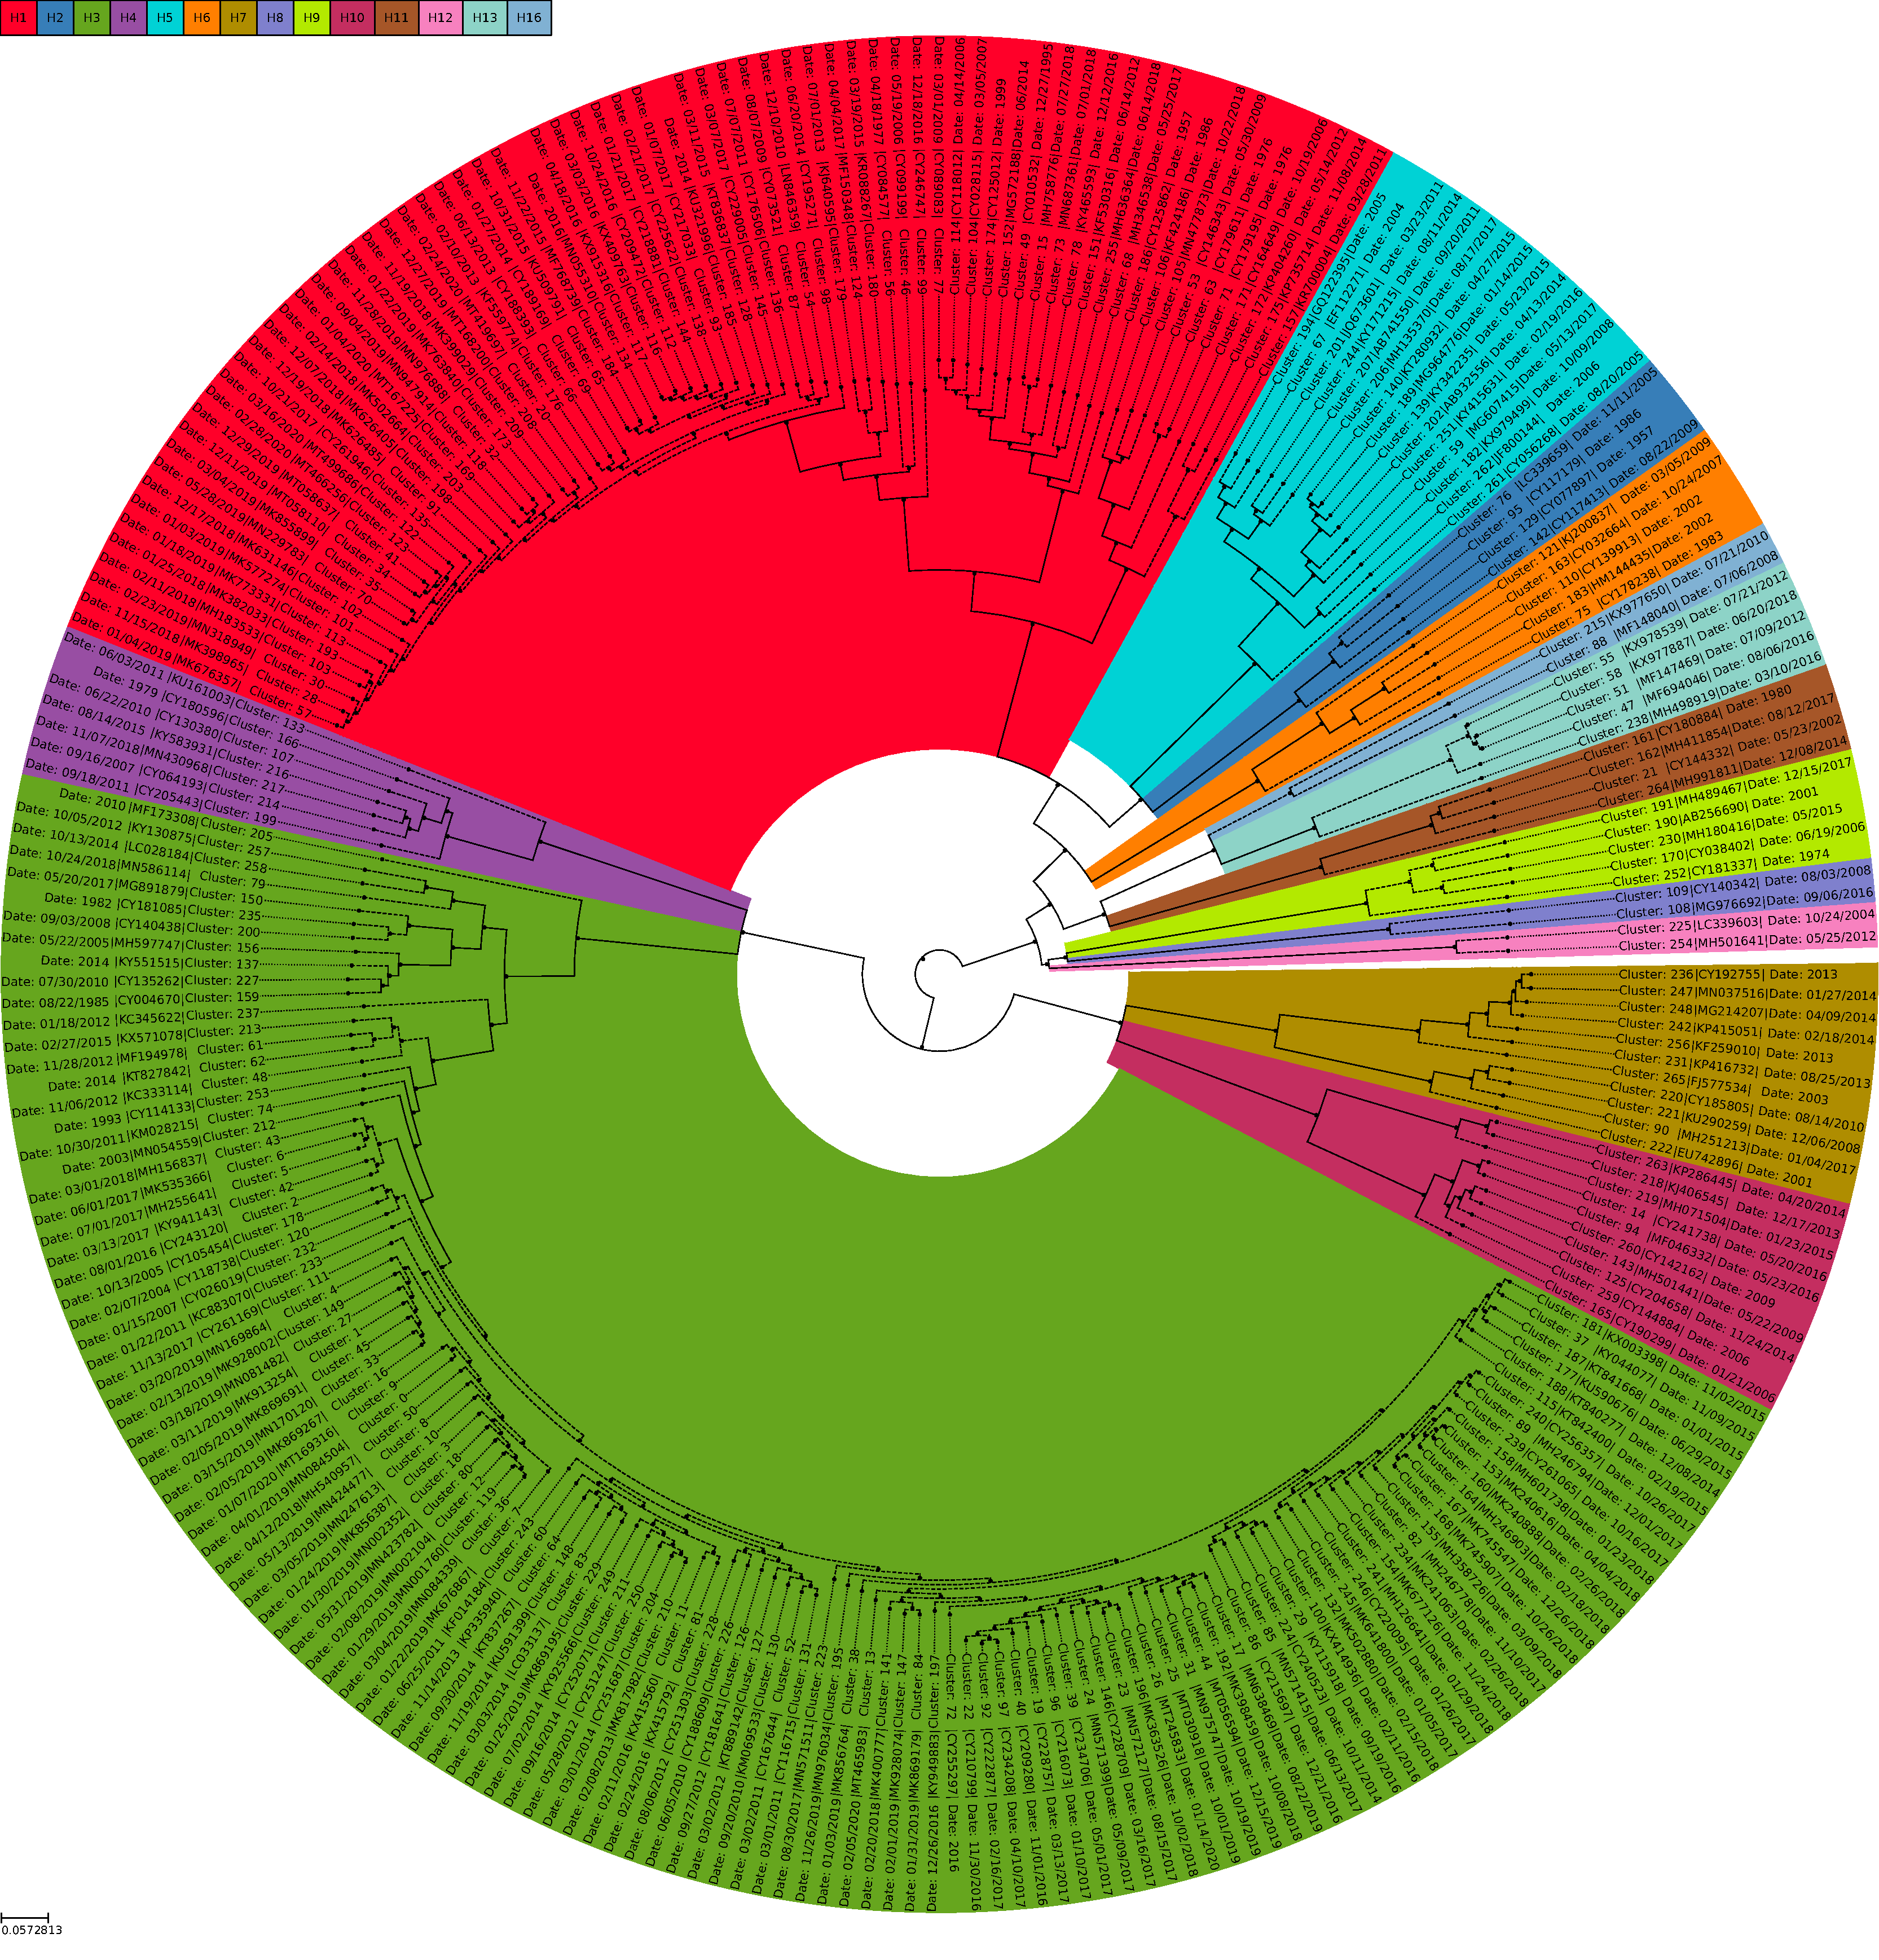
\includegraphics[width=\textwidth]{UMAP/Guidetree_segment_4_H_Centroid.pdf}
%     \caption[Centroid guidetree of segment 4 with UK]{\textbf{Centroid guidetree of segment 4 with UK.} }
%     \label{fig:UMAP_Guidetree_Centroid_4}
% \end{figure}

% \FloatBarrier

% \begin{figure}[!hbt]
%     \centering
%     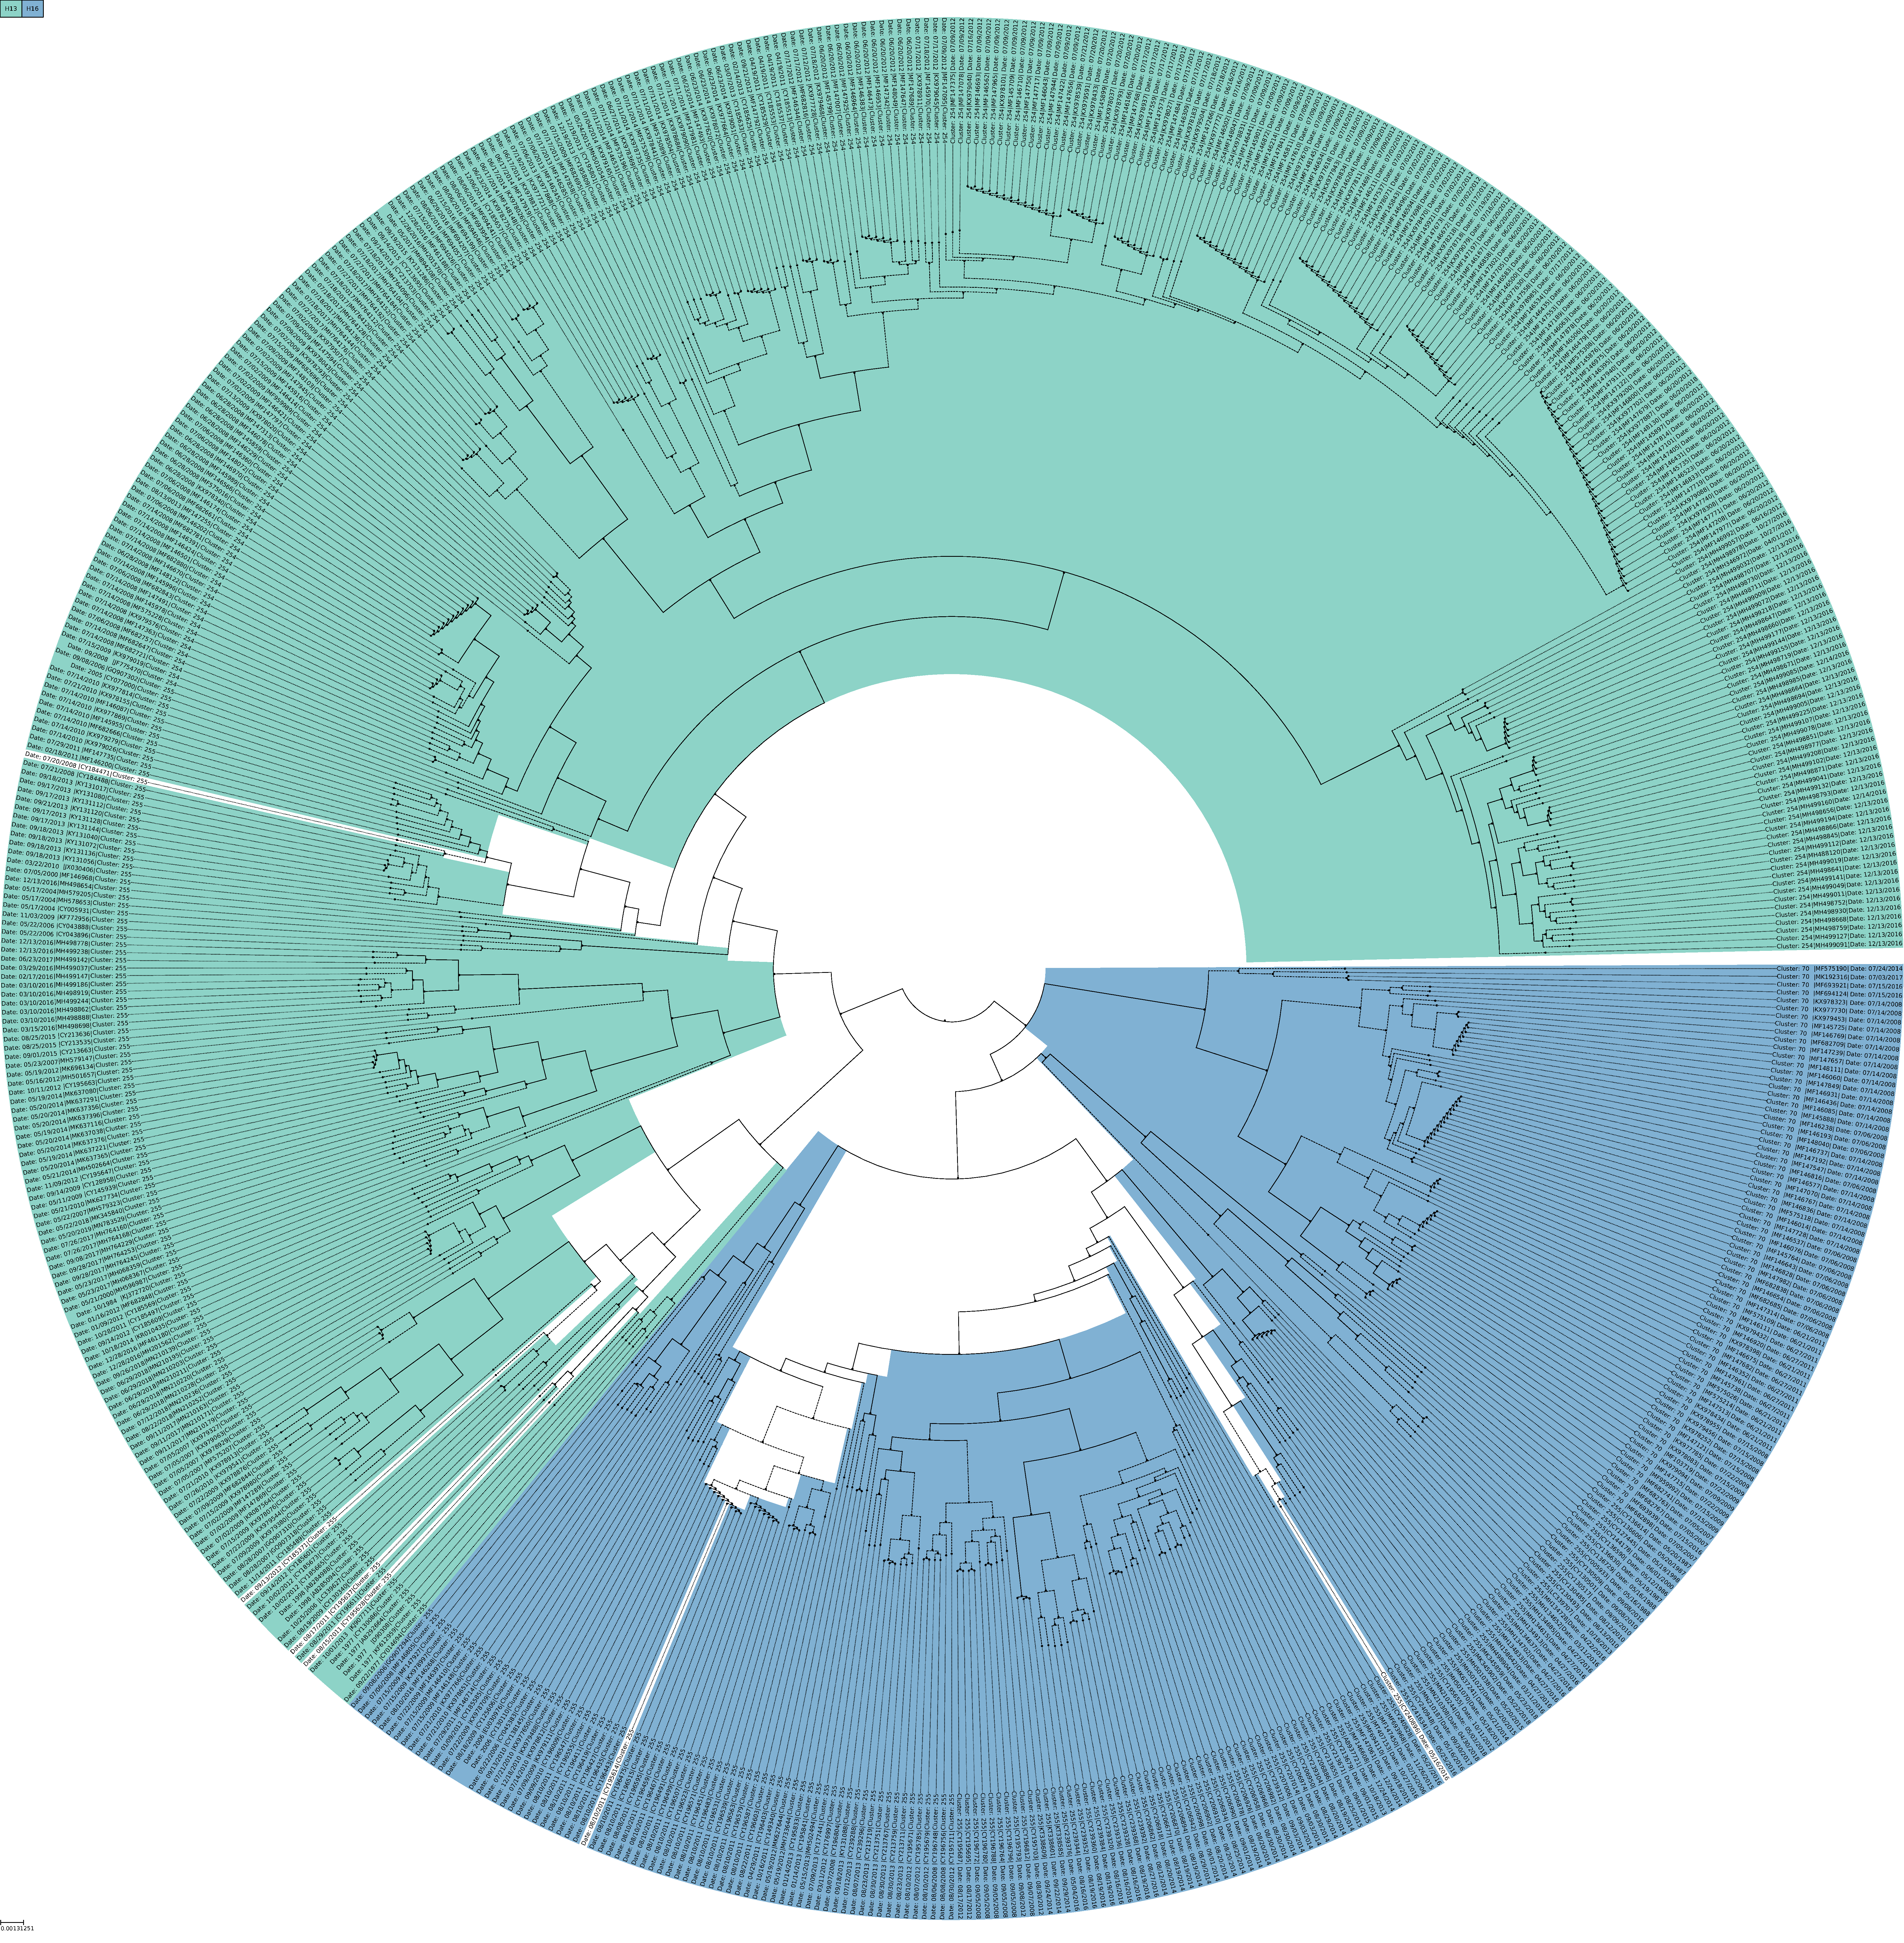
\includegraphics[width=\textwidth]{UMAP/Precalculated_Segment_4_H_Euclidean.pdf}
%     \caption[UPGMA tree of H13/H16 with euclidean distance]{\textbf{UPGMA tree of H13/H16 with euclidean distance.} .}
%     \label{fig:Precalculated_Euclid}
% \end{figure}

% \FloatBarrier

% \begin{figure}[!hbt]
%     \centering
%     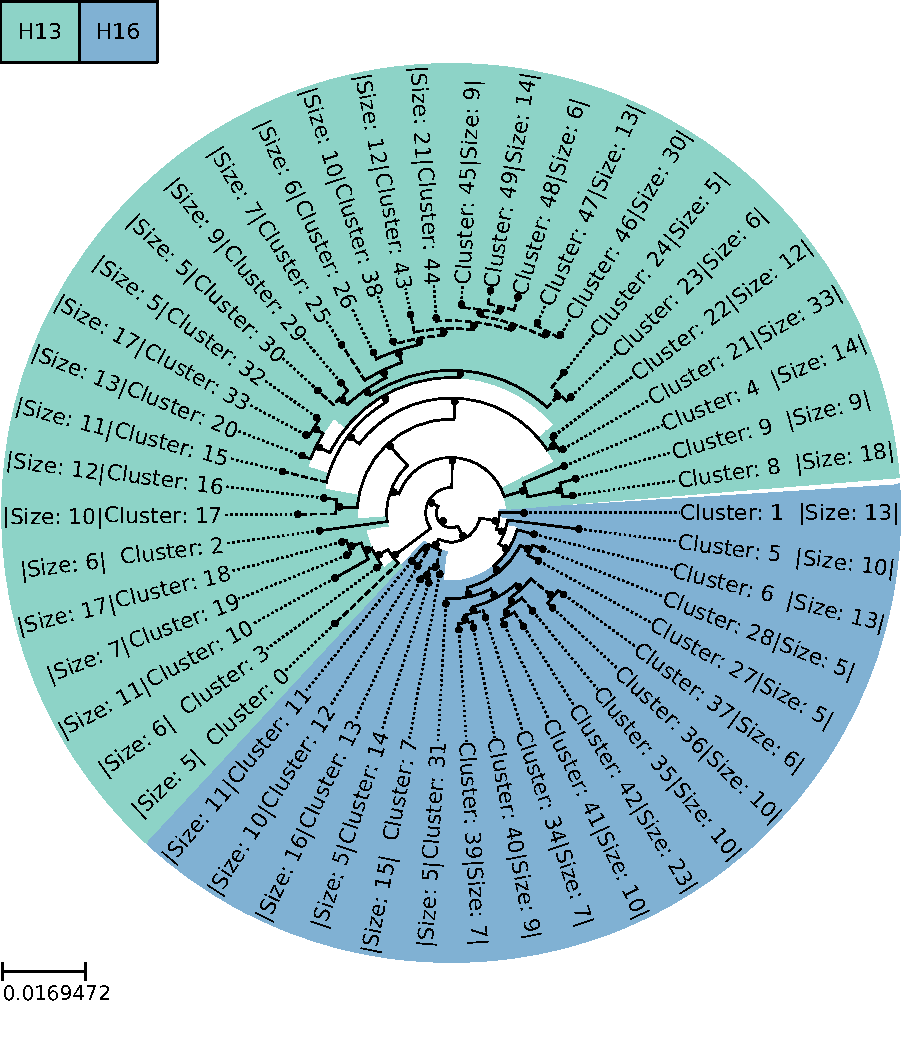
\includegraphics[width=\textwidth]{PCA/Clustertree_Segment_4_H_Euclidean.pdf}
%     \caption[Simple clustering tree of H13/H16 with euclidean distance]{\textbf{Simple clustering tree of H13/H16 with euclidean distance.} .}
%     \label{fig:Simple_Clustertree_Euclid}
% \end{figure}

\FloatBarrier
\newpage

\begin{figure}[!hbt]
    \centering
    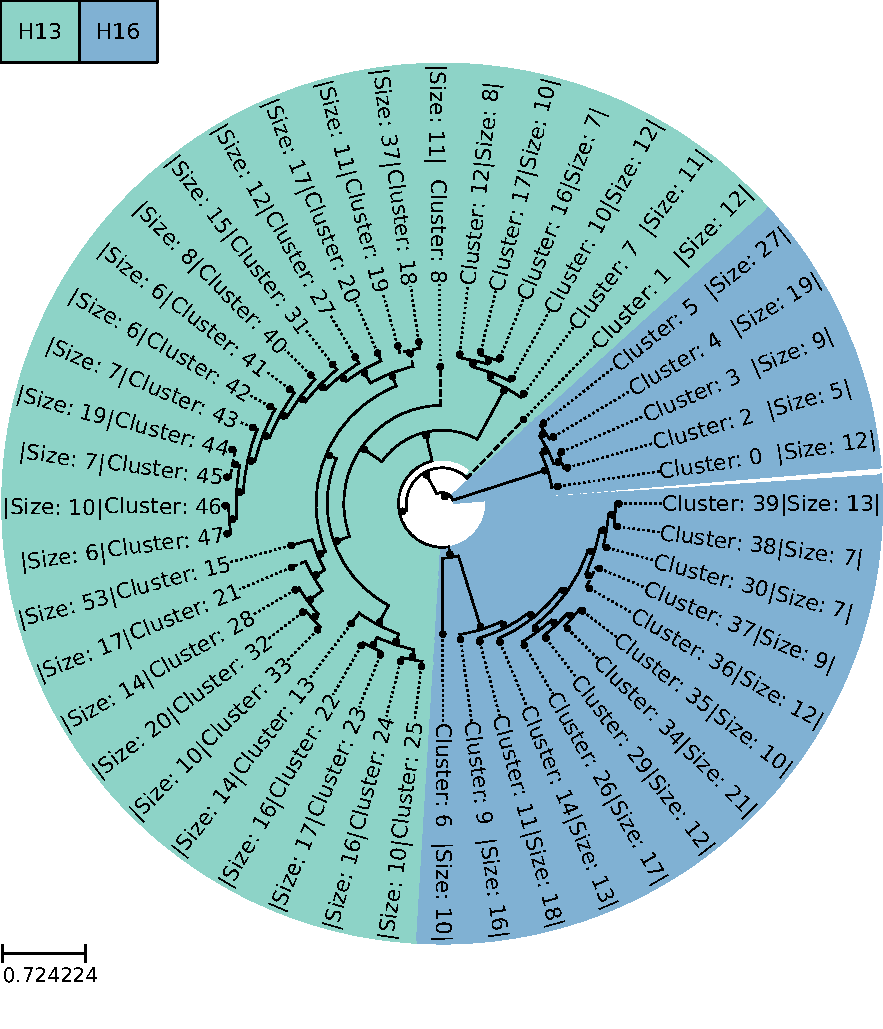
\includegraphics[width=\textwidth]{UMAP/Clustertree_Segment_4_H_Simple.pdf}
    \caption[Simple clustering tree of H13/H16 with UMAP]{\textbf{Simple clustering tree of H13/H16 with UMAP.} Cluster tree based on the clustering by simple \texttt{HDBSCAN} without any $\varepsilon$ exploration and hybrid clustering. The used vectors were calculated from the sequences, present in the H13 and H16 clusters in \autoref{fig:PCA_Clusteree_Knee_4} with prior \texttt{PCA} reduction to 100 and \texttt{UMAP} reduction to 30 dimensions. On both sides of the tree, subtrees of H16 are first joined to subtrees of H13 before joining together and to another H13 subtree afterwards. Therefore, no clear separation is present.}
    \label{fig:Simple_Clustertree_UMAP}
\end{figure}

\FloatBarrier
\newpage

\begin{table}[!hbt]
    \centering
    \caption[Clustering results]{\textbf{Clustering results.} The results of the final clustering using the combination of the \texttt{PCA} reduction and the Kneedle Algorithm . Listed is every used segment with the number of raw clusters and the final cluster number after hybrid clustering with the given value of $\varepsilon$. The numbers of mixed cluster numbers of H and N denotes number of clusters containing vectors related to more than one subtype. The variance is calculated as the sum of the explained variance by the \texttt{PCA}.}
    \label{tab:Result_Cluster}
    \pgfplotstabletypeset[
        every head row/.style={
            before row={
                \toprule
                & \multicolumn{3}{l}{\textbf{\#Cluster}} & \multicolumn{2}{l}{\textbf{\#Mixed}} & &\\
                \cmidrule(lr){2-4}\cmidrule(lr){5-6}
            },
            after row={
                \midrule
            },
        },
        every last row/.style={
            after row={
                %... & ... & ... & ... & ... & ... & ... & ...\\
                \bottomrule
            },
        },
        begin table=\begin{tabular*}{\textwidth},
        end table=\end{tabular*},
        columns={0,1,2,3,5,6,4,7,8},
        columns/0/.style={int detect, multicolumn names=l,column name=\textbf{Segment}, column type=@{\extracolsep{\fill}\hspace{6pt}}r},
        columns/1/.style={int detect, multicolumn names=l,column name=\textbf{Final}, column type=r},
        columns/2/.style={int detect, multicolumn names=l,column name=\textbf{Raw}, column type=r},
        columns/3/.style={multicolumn names=l,column name=\textbf{Normalized}, column type=r},
        columns/4/.style={int detect, multicolumn names=l,column name=\textbf{\#Unclustered}, column type=r},
        columns/5/.style={int detect, multicolumn names=l,column name=\textbf{H}, column type=r},
        columns/6/.style={int detect, multicolumn names=l,column name=\textbf{N}, column type=r},
        columns/7/.style={multicolumn names=l,column name=\textbf{$\varepsilon$}, column type=r},
        columns/8/.style={multicolumn names=l,column name=\textbf{$\text{Var}(X)$}, column type=r},
    ]
    {Results/information.csv}
\end{table}

% \begin{table}[!hbt]
%     \centering
%     \caption[Cluster database]{\textbf{Cluster database.}.}
%     \label{tab:Result_Database}
%     \pgfplotstabletypeset[
%         every head row/.style={
%             before row={
%                 \toprule
%             },
%             after row={
%                 \midrule
%             },
%         },
%         every last row/.style={
%             after row={
%                 ... & ... & ... & ... & ... & ... & ... \\
%                 \bottomrule
%             },
%         },
%         begin table=\begin{tabular*}{\textwidth},
%         end table=\end{tabular*},
%         columns={0,1,2,3,4,5,6},
%         columns/0/.style={string type,multicolumn names=l,column name=\textbf{Accession}, column type=@{\extracolsep{\fill}\hspace{6pt}}r},
%         columns/1/.style={int detect, multicolumn names=l,column name=\textbf{Segment}, column type=r},
%         columns/2/.style={int detect, multicolumn names=l,column name=\textbf{Cluster}, column type=r},
%         columns/3/.style={string type,multicolumn names=l,column name=\textbf{H}, column type=r},
%         columns/4/.style={string type,multicolumn names=l,column name=\textbf{Centroid}, column type=r},
%         columns/5/.style={string type,multicolumn names=l,column name=\textbf{N}, column type=r},
%         columns/6/.style={string type,multicolumn names=l,column name=\textbf{Strain}, column type=r},
%     ]
%     {Graphics/cluster_head.csv}
% \end{table}

% \newpage

% \begin{figure}[!hbt]
%     \centering
%     \begin{subfigure}[b]{0.475\textwidth}
%         \caption[Kneedle Algorithm]{\textbf{Kneedle Algorithm}}
%         \label{subfig:Result_Cluster_Knee_Kneedle_1}            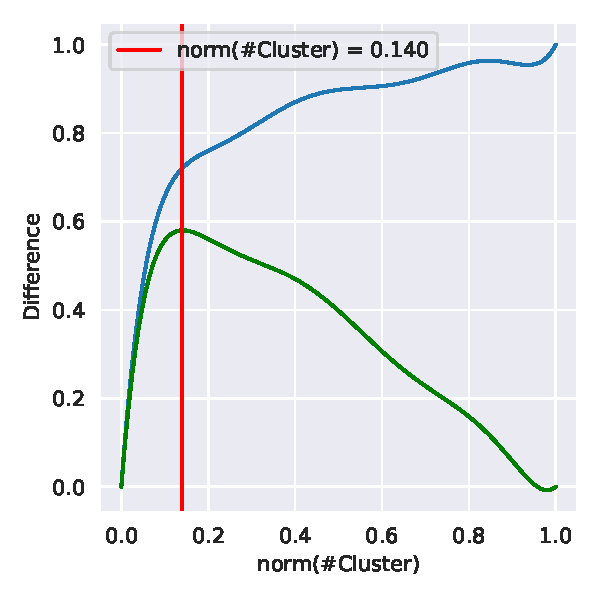
\includegraphics[width=\textwidth]{Results/Cluster_Knee_Segment_1.pdf}
%     \end{subfigure}
%     \hfill
%     \begin{subfigure}[b]{0.475\textwidth}
%         \caption[Kneedle point]{\textbf{Knee Point}}
%         \label{subfig:Result_Cluster_Knee_Elbow_1}            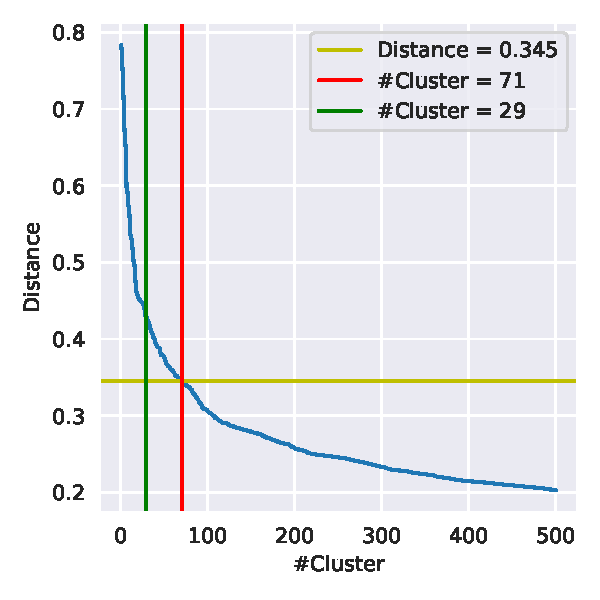
\includegraphics[width=\textwidth]{Results/Cluster_Elbow_Knee_Segment_1.pdf}
%     \end{subfigure}
%     \vskip\baselineskip
%     \begin{subfigure}[b]{0.475\textwidth}
%         \caption[Cluster distribution]{\textbf{Cluster distribution}}
%         \label{subfig:Result_Cluster_Knee_Distributione_1}            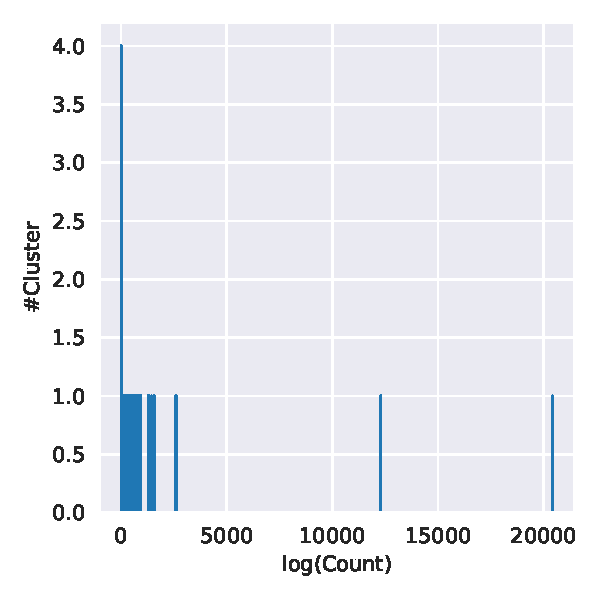
\includegraphics[width=\textwidth]{Results/Cluster_Distribution_Segment_1.pdf}
%     \end{subfigure}
%     \hfill
%     \begin{subfigure}[b]{0.475\textwidth}
%         \caption[Logarithmic distribution]{\textbf{Logarithmic distribution}}
%         \label{subfig:Result_Cluster_Knee_Distribution_log_1}            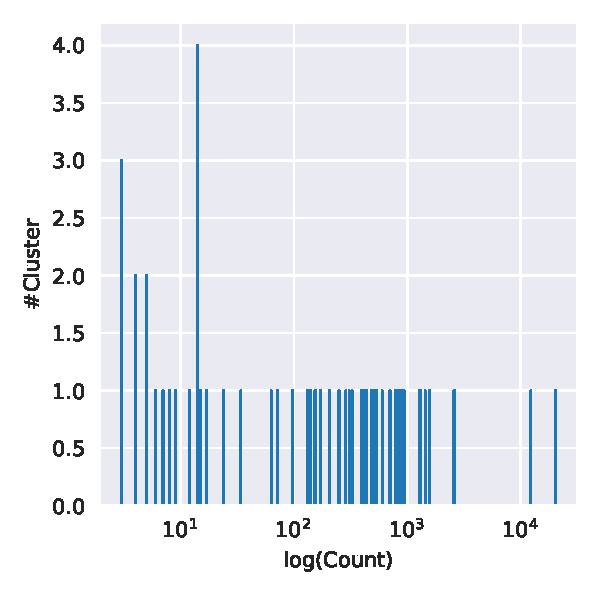
\includegraphics[width=\textwidth]{Results/Cluster_Distribution_Log_Segment_1.pdf}
%     \end{subfigure}
%     \caption[Clustering of segment 1]{\textbf{Clustering of segment 1.} }
%     \label{fig:Result_Cluster_Knee_1}
% \end{figure}

% \newpage

% \begin{figure}[!hbt]
%     \centering
%     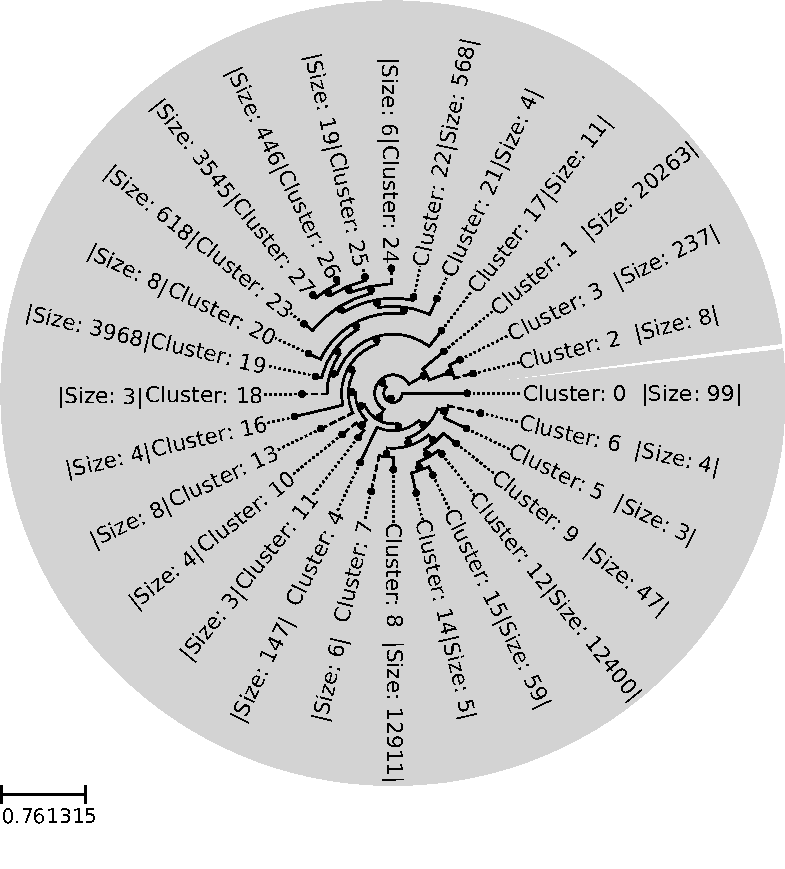
\includegraphics[width=\textwidth]{Results/Clustertree_Segment_1.pdf}
%     \caption[Clustering tree of segment 1]{\textbf{Clustering tree of segment 1.} }
%     \label{fig:Result_Clustertree_Segment_1}
% \end{figure}

% \newpage

% \begin{figure}[!hbt]
%     \centering
%     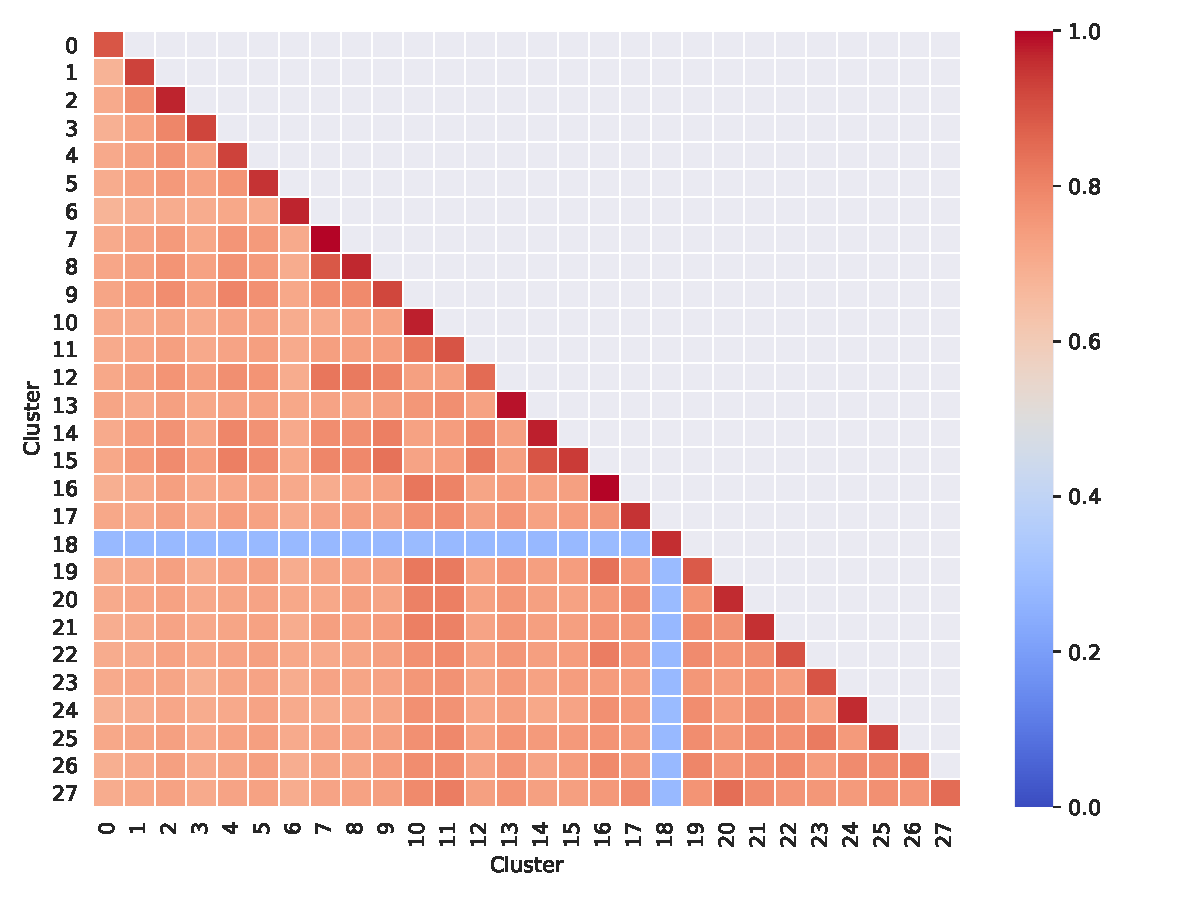
\includegraphics[width=\textwidth]{Results/Cluster_Difference_Segment_1.pdf}
%     \caption[Similarity matrix of segment 1 clusters]{\textbf{Similarity matrix of segment 1 clusters.} }
%     \label{fig:Proof_Clustertree_Segment_1}
% \end{figure}

% \newpage

% \begin{figure}[!hbt]
%     \centering
%     \begin{subfigure}[b]{0.475\textwidth}
%         \caption[Kneedle Algorithm]{\textbf{Kneedle Algorithm}}
%         \label{subfig:Result_Cluster_Knee_Kneedle_2}            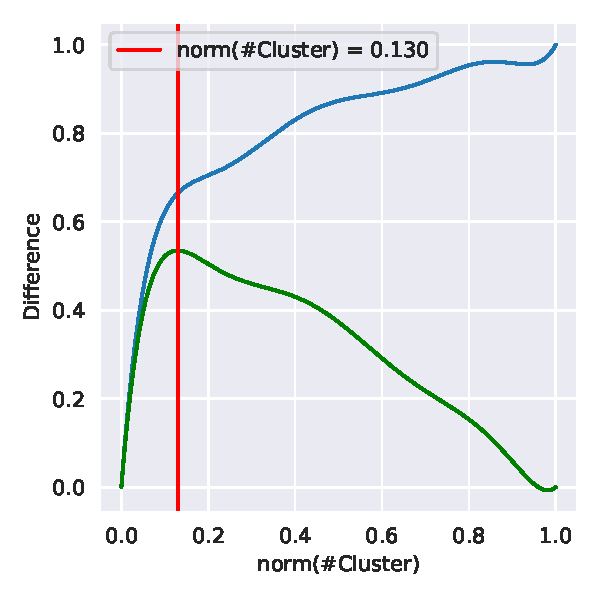
\includegraphics[width=\textwidth]{Results/Cluster_Knee_Segment_2.pdf}
%     \end{subfigure}
%     \hfill
%     \begin{subfigure}[b]{0.475\textwidth}
%         \caption[Kneedle point]{\textbf{Knee point}}
%         \label{subfig:Result_Cluster_Knee_Elbow_2}            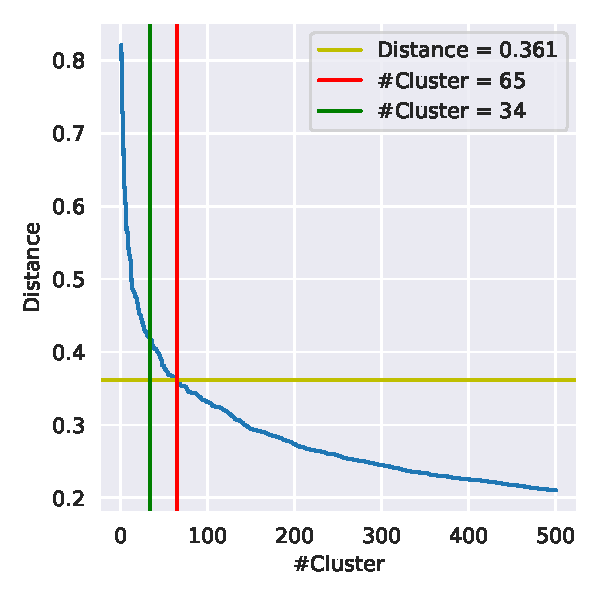
\includegraphics[width=\textwidth]{Results/Cluster_Elbow_Knee_Segment_2.pdf}
%     \end{subfigure}
%     \vskip\baselineskip
%     \begin{subfigure}[b]{0.475\textwidth}
%         \caption[Cluster distribution]{\textbf{Cluster distribution}}
%         \label{subfig:Result_Cluster_Knee_Distributione_2}            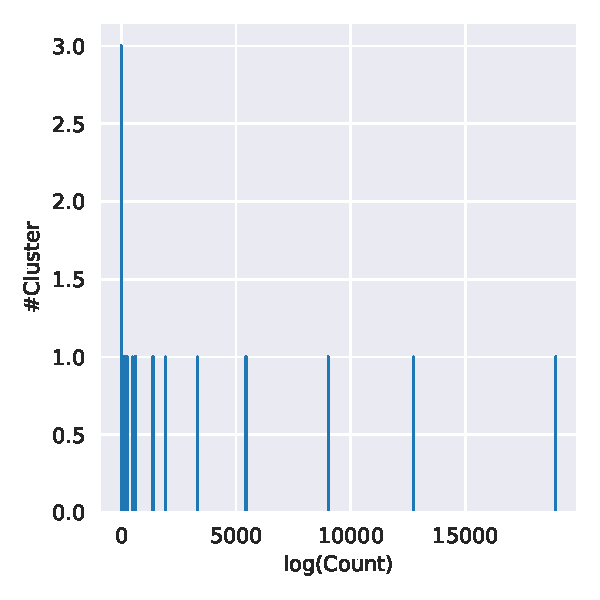
\includegraphics[width=\textwidth]{Results/Cluster_Distribution_Segment_2.pdf}
%     \end{subfigure}
%     \hfill
%     \begin{subfigure}[b]{0.475\textwidth}
%         \caption[Logarithmic distribution]{\textbf{Logarithmic distribution}}
%         \label{subfig:Result_Cluster_Knee_Distribution_log_2}            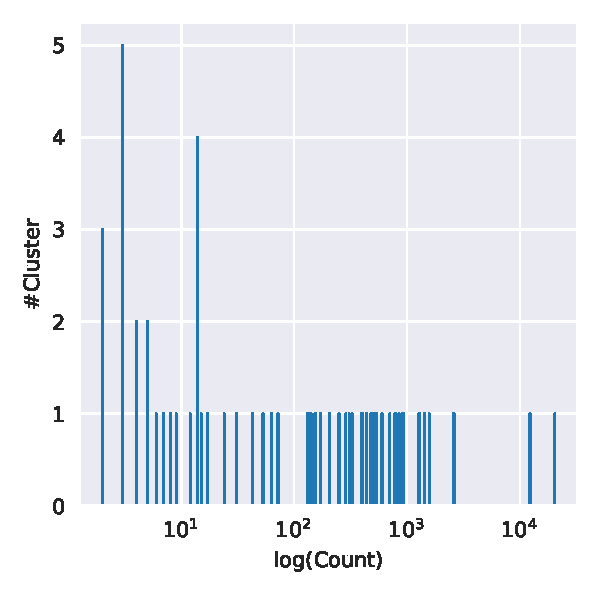
\includegraphics[width=\textwidth]{Results/Cluster_Distribution_Log_Segment_2.pdf}
%     \end{subfigure}
%     \caption[Clustering of segment 2]{\textbf{Clustering of segment 2.} }
%     \label{fig:Result_Cluster_Knee_2}
% \end{figure}

% \newpage

% \begin{figure}[!hbt]
%     \centering
%     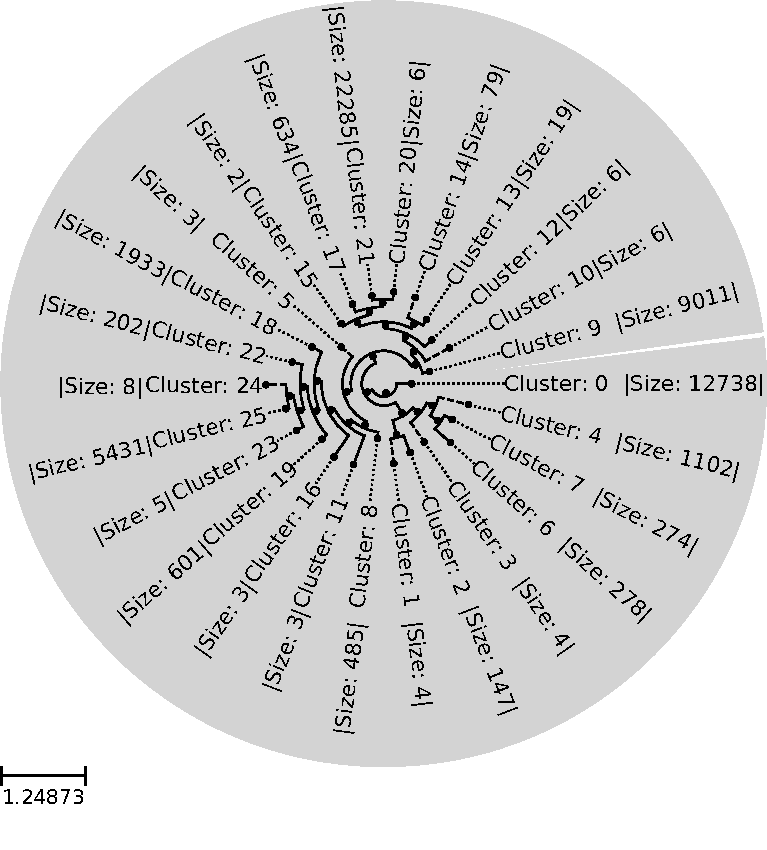
\includegraphics[width=\textwidth]{Results/Clustertree_Segment_2.pdf}
%     \caption[Clustering tree of segment 2]{\textbf{Clustering tree of segment 2.} }
%     \label{fig:Result_Clustertree_Segment_2}
% \end{figure}

% \newpage

% \begin{figure}[!hbt]
%     \centering
%     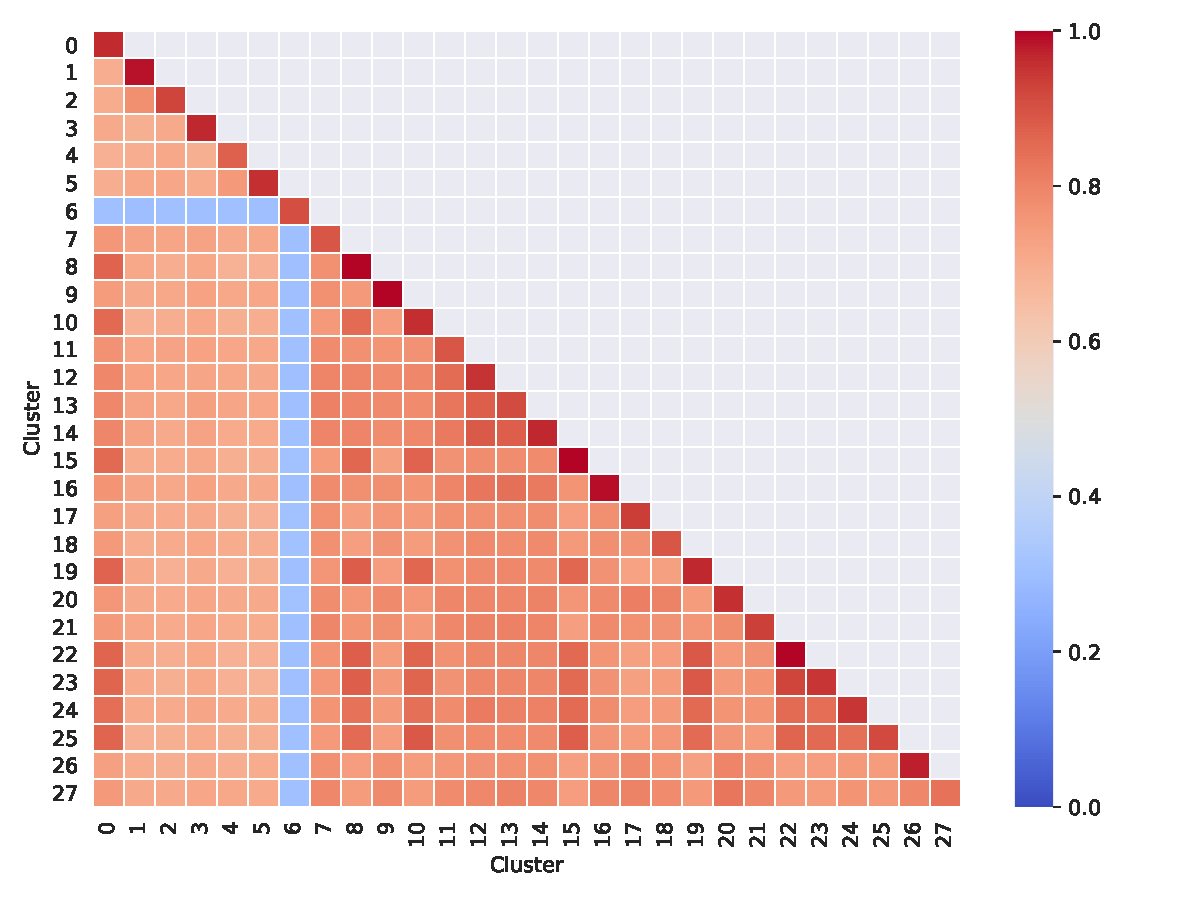
\includegraphics[width=\textwidth]{Results/Cluster_Difference_Segment_2.pdf}
%     \caption[Similarity matrix of segment 2 clusters]{\textbf{Similarity matrix of segment 2 clusters.} }
%     \label{fig:Proof_Clustertree_Segment_2}
% \end{figure}

% \newpage

% \begin{figure}[!hbt]
%     \centering
%     \begin{subfigure}[b]{0.475\textwidth}
%         \caption[Kneedle Algorithm]{\textbf{Kneedle Algorithm}}
%         \label{subfig:Result_Cluster_Knee_Kneedle_3}            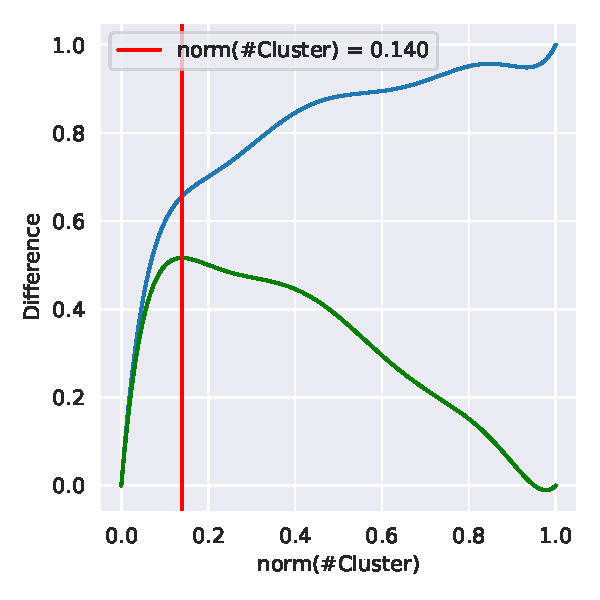
\includegraphics[width=\textwidth]{Results/Cluster_Knee_Segment_3.pdf}
%     \end{subfigure}
%     \hfill
%     \begin{subfigure}[b]{0.475\textwidth}
%         \caption[Kneedle point]{\textbf{Knee point}}
%         \label{subfig:Result_Cluster_Knee_Elbow_3}            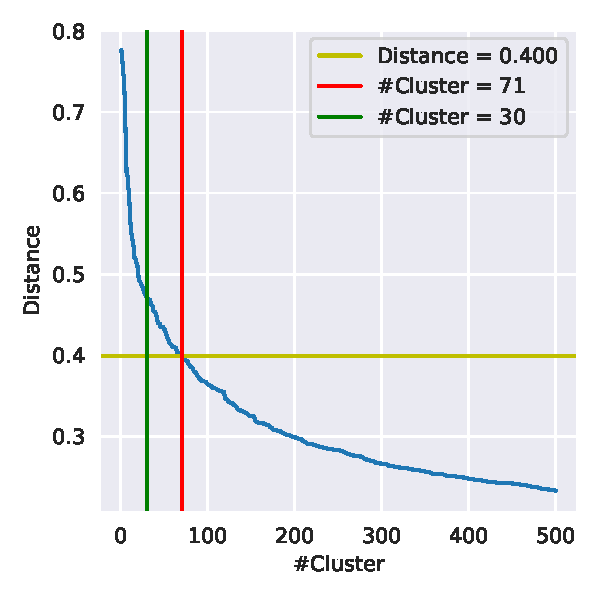
\includegraphics[width=\textwidth]{Results/Cluster_Elbow_Knee_Segment_3.pdf}
%     \end{subfigure}
%     \vskip\baselineskip
%     \begin{subfigure}[b]{0.475\textwidth}
%         \caption[Cluster distribution]{\textbf{Cluster distribution}}
%         \label{subfig:Result_Cluster_Knee_Distributione_3}            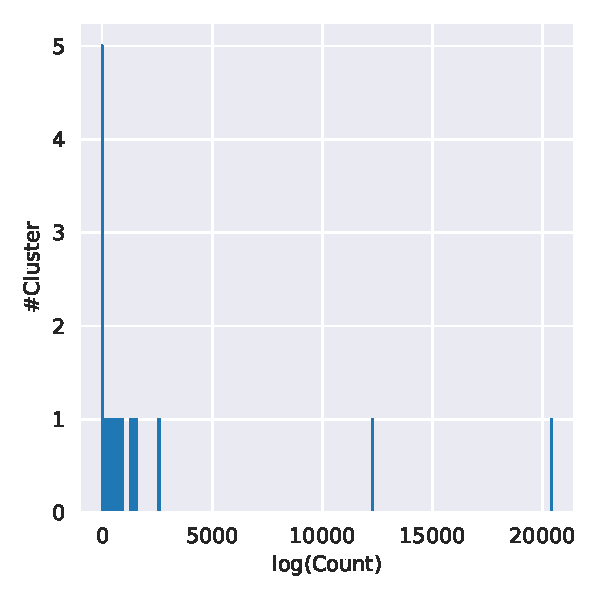
\includegraphics[width=\textwidth]{Results/Cluster_Distribution_Segment_3.pdf}
%     \end{subfigure}
%     \hfill
%     \begin{subfigure}[b]{0.475\textwidth}
%         \caption[Logarithmic distribution]{\textbf{Logarithmic distribution}}
%         \label{subfig:Result_Cluster_Knee_Distribution_log_3}            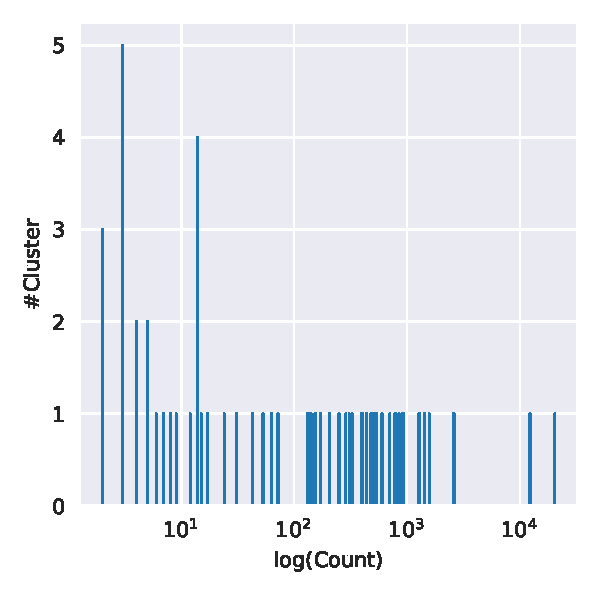
\includegraphics[width=\textwidth]{Results/Cluster_Distribution_Log_Segment_3.pdf}
%     \end{subfigure}
%     \caption[Clustering of segment 3]{\textbf{Clustering of segment 3.} }
%     \label{fig:Result_Cluster_Knee_3}
% \end{figure}

% \newpage

% \begin{figure}[!hbt]
%     \centering
%     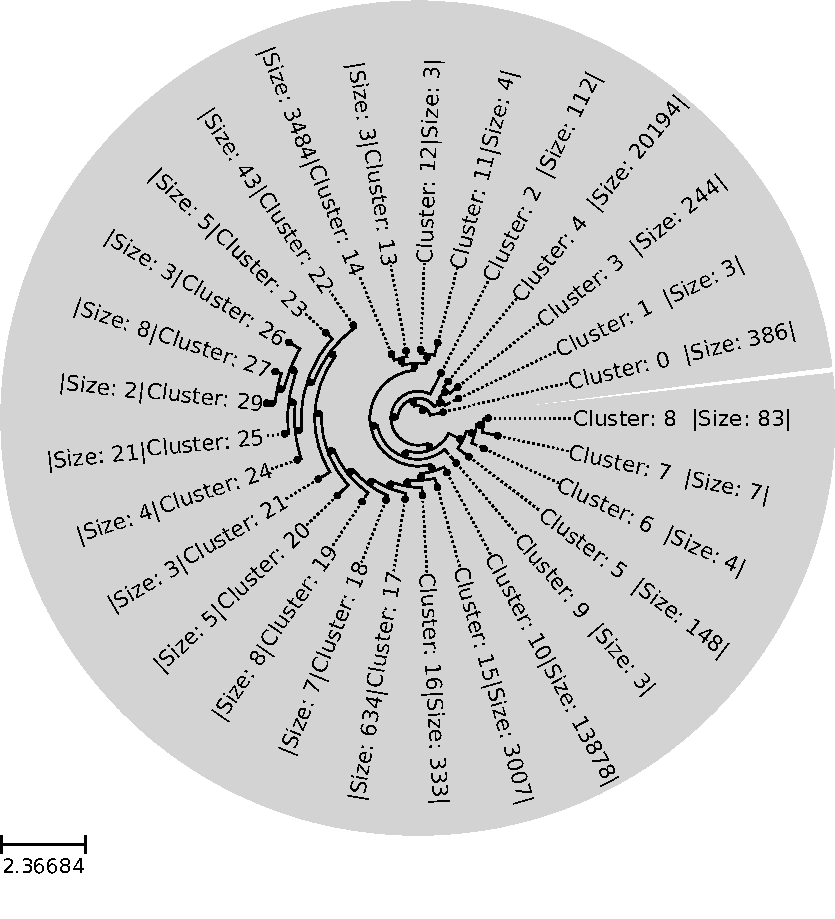
\includegraphics[width=\textwidth]{Results/Clustertree_Segment_3.pdf}
%     \caption[Clustering tree of segment 3]{\textbf{Clustering tree of segment 3.} }
%     \label{fig:Result_Clustertree_Segment_3}
% \end{figure}

% \newpage

% \begin{figure}[!hbt]
%     \centering
%     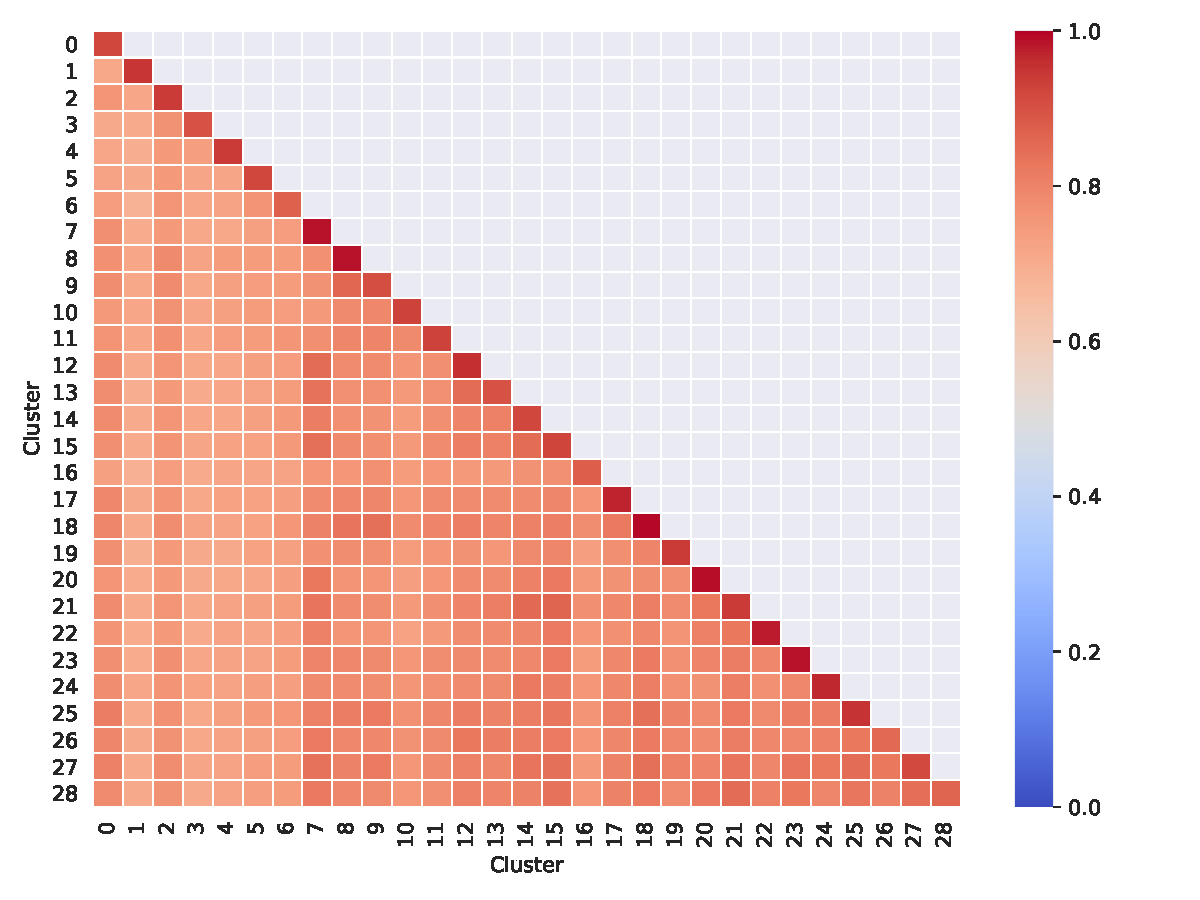
\includegraphics[width=\textwidth]{Results/Cluster_Difference_Segment_3.pdf}
%     \caption[Similarity matrix of segment 3 clusters]{\textbf{Similarity matrix of segment 3 clusters.} }
%     \label{fig:Proof_Clustertree_Segment_3}
% \end{figure}

\FloatBarrier
\newpage

\begin{figure}[!hbt]
    \centering
    \begin{subfigure}[b]{0.475\textwidth}
        \caption[Kneedle Algorithm]{\textbf{Kneedle Algorithm}}
        \label{subfig:Result_Cluster_Knee_Kneedle_4}            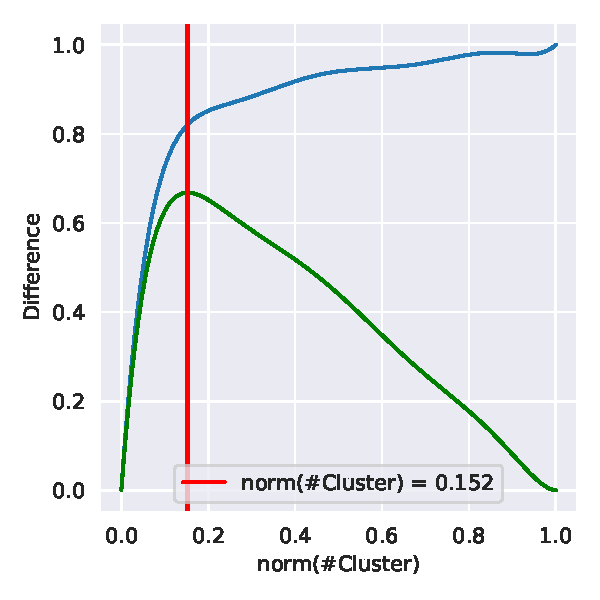
\includegraphics[width=\textwidth]{Results/Cluster_Knee_Segment_4.pdf}
    \end{subfigure}
    \hfill
    \begin{subfigure}[b]{0.475\textwidth}
        \caption[Kneedle point]{\textbf{Knee Point}}
        \label{subfig:Result_Cluster_Knee_Elbow_4}            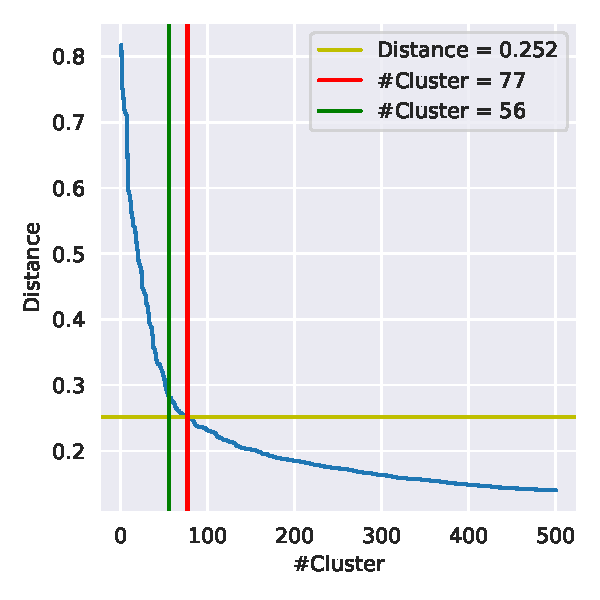
\includegraphics[width=\textwidth]{Results/Cluster_Elbow_Knee_Segment_4.pdf}
    \end{subfigure}
    \vskip\baselineskip
    \begin{subfigure}[b]{0.475\textwidth}
        \caption[Cluster distribution]{\textbf{Cluster distribution}}
        \label{subfig:Result_Cluster_Knee_Distributione_4}            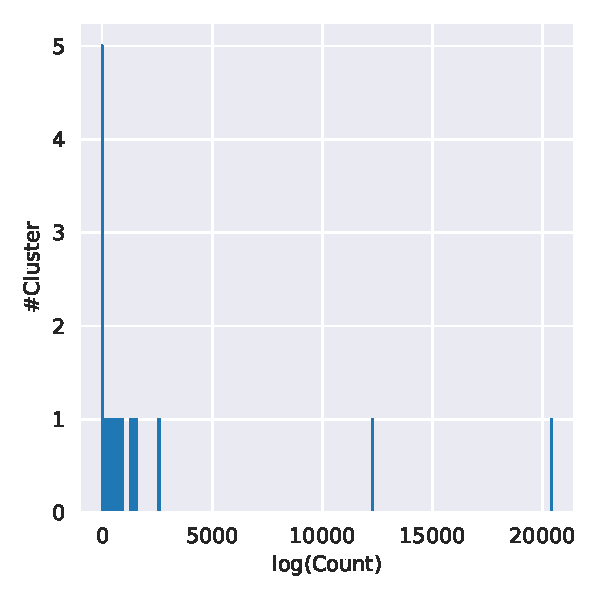
\includegraphics[width=\textwidth]{Results/Cluster_Distribution_Segment_4.pdf}
    \end{subfigure}
    \hfill
    \begin{subfigure}[b]{0.475\textwidth}
        \caption[Logarithmic distribution]{\textbf{Logarithmic distribution}}
        \label{subfig:Result_Cluster_Knee_Distribution_log_4}            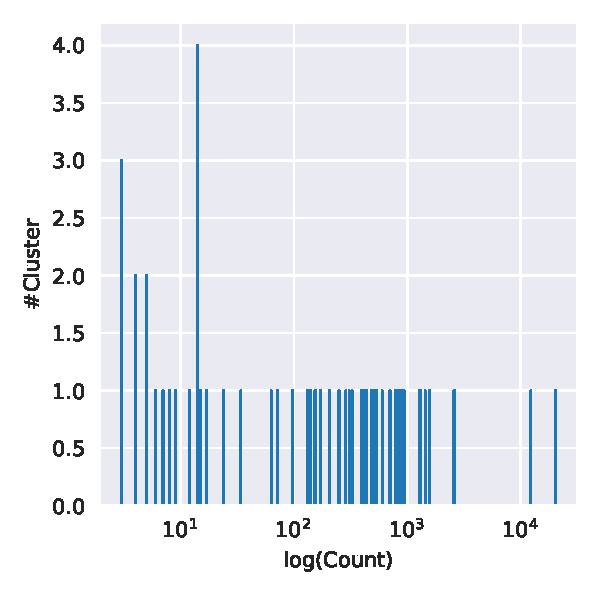
\includegraphics[width=\textwidth]{Results/Cluster_Distribution_Log_Segment_4.pdf}
    \end{subfigure}
    \caption[Clustering of segment 4]{\textbf{Clustering of segment 4.} Segment 4 clustering, using the combination of \texttt{PCA} with 50 extracted components and the Kneedle Algorithm results in the given figure. The green curve in the top left sub figure describes the change of the distance in the single linkage tree with increasing normalized cluster number and, therefore, the location of the knee, at the maximum, highlighted by the red line. The blue line is the inverse polynomial representation of the blue line in top right sub figure. The top right sub figure shows the absolute relation of the distance in the single linkage tree to the total number of clusters as the blue line. The red line, indicates the number of raw clusters, by the \texttt{DBSCAN} part of the hybrid \texttt{HDBSCAN} clustering and the final cluster number in green. The yellow line describes the threshold, extracted from the knee and, therefore, the $\varepsilon$ value used to perform the hybrid clustering. The normalized cluster number in the red line in the top left sub figure is equivalent to the raw cluster number in the top right sub figure. The bottom sub figures give information about the distribution of the clusters sizes, by plotting the number of clusters containing a given counted number of sequences in continuous and logarithmic scale.}
    \label{fig:Result_Cluster_Knee_4}
\end{figure}

% \newpage

% \begin{figure}[!hbt]
%     \centering
%     \begin{subfigure}[b]{0.475\textwidth}
%         \caption[Kneedle Algorithm]{\textbf{Kneedle Algorithm}}
%         \label{subfig:Result_Cluster_Knee_Kneedle_5}            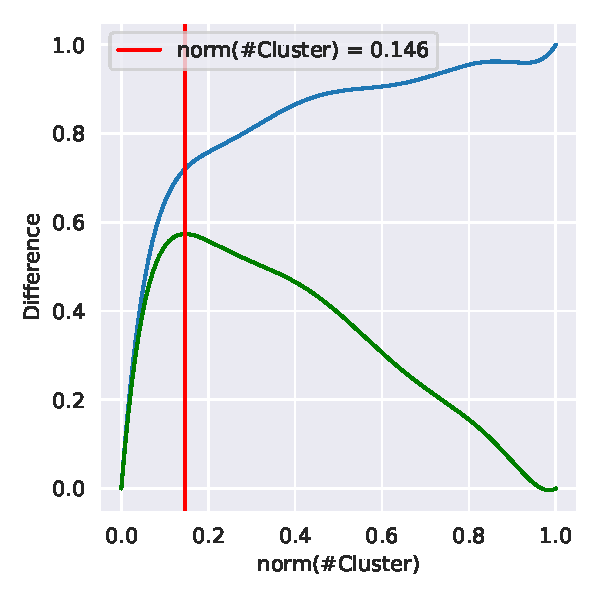
\includegraphics[width=\textwidth]{Results/Cluster_Knee_Segment_5.pdf}
%     \end{subfigure}
%     \hfill
%     \begin{subfigure}[b]{0.475\textwidth}
%         \caption[Kneedle point]{\textbf{Knee point}}
%         \label{subfig:Result_Cluster_Knee_Elbow_5}            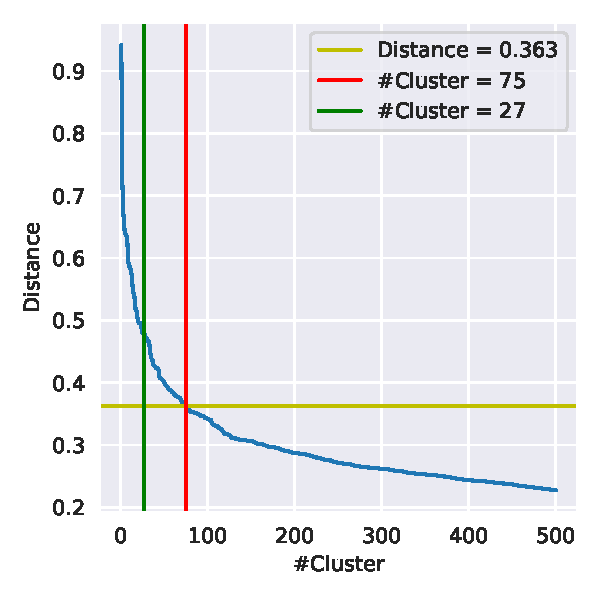
\includegraphics[width=\textwidth]{Results/Cluster_Elbow_Knee_Segment_5.pdf}
%     \end{subfigure}
%     \vskip\baselineskip
%     \begin{subfigure}[b]{0.475\textwidth}
%         \caption[Cluster distribution]{\textbf{Cluster distribution}}
%         \label{subfig:Result_Cluster_Knee_Distributione_5}            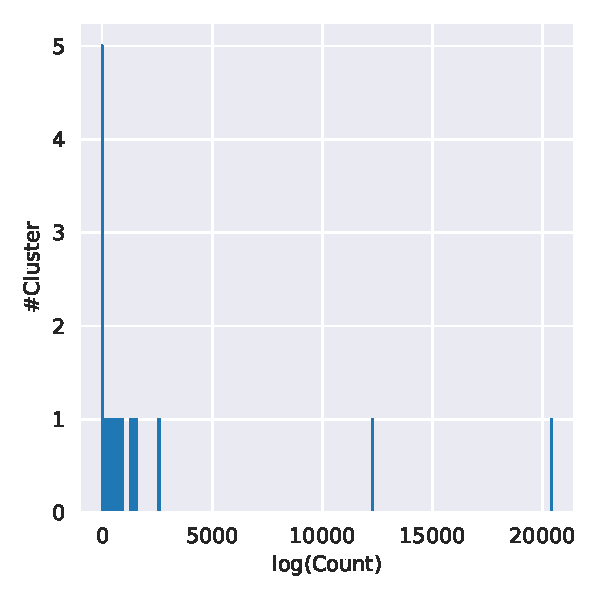
\includegraphics[width=\textwidth]{Results/Cluster_Distribution_Segment_5.pdf}
%     \end{subfigure}
%     \hfill
%     \begin{subfigure}[b]{0.475\textwidth}
%         \caption[Logarithmic distribution]{\textbf{Logarithmic distribution}}
%         \label{subfig:Result_Cluster_Knee_Distribution_log_5}            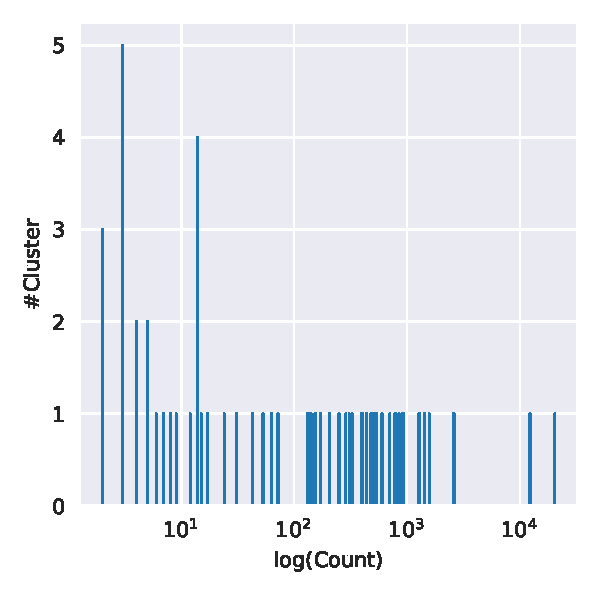
\includegraphics[width=\textwidth]{Results/Cluster_Distribution_Log_Segment_5.pdf}
%     \end{subfigure}
%     \caption[Clustering of segment 5]{\textbf{Clustering of segment 5.} }
%     \label{fig:Result_Cluster_Knee_5}
% \end{figure}

% \newpage

% \begin{figure}[!hbt]
%     \centering
%     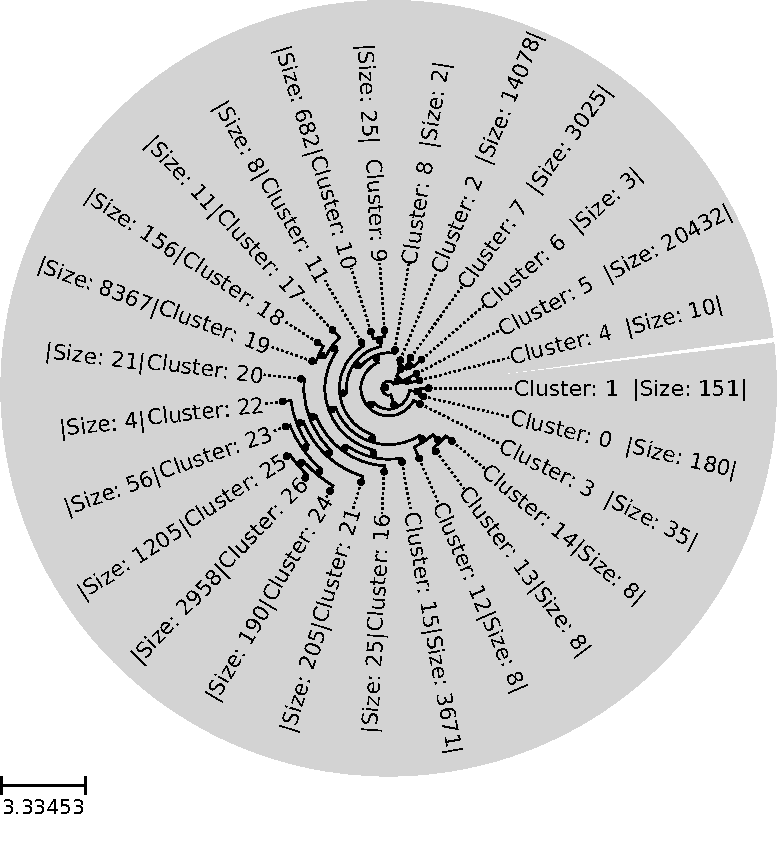
\includegraphics[width=\textwidth]{Results/Clustertree_Segment_5.pdf}
%     \caption[Clustering tree of segment 5]{\textbf{Clustering tree of segment 5.} }
%     \label{fig:Result_Clustertree_Segment_5}
% \end{figure}

% \newpage

% \begin{figure}[!hbt]
%     \centering
%     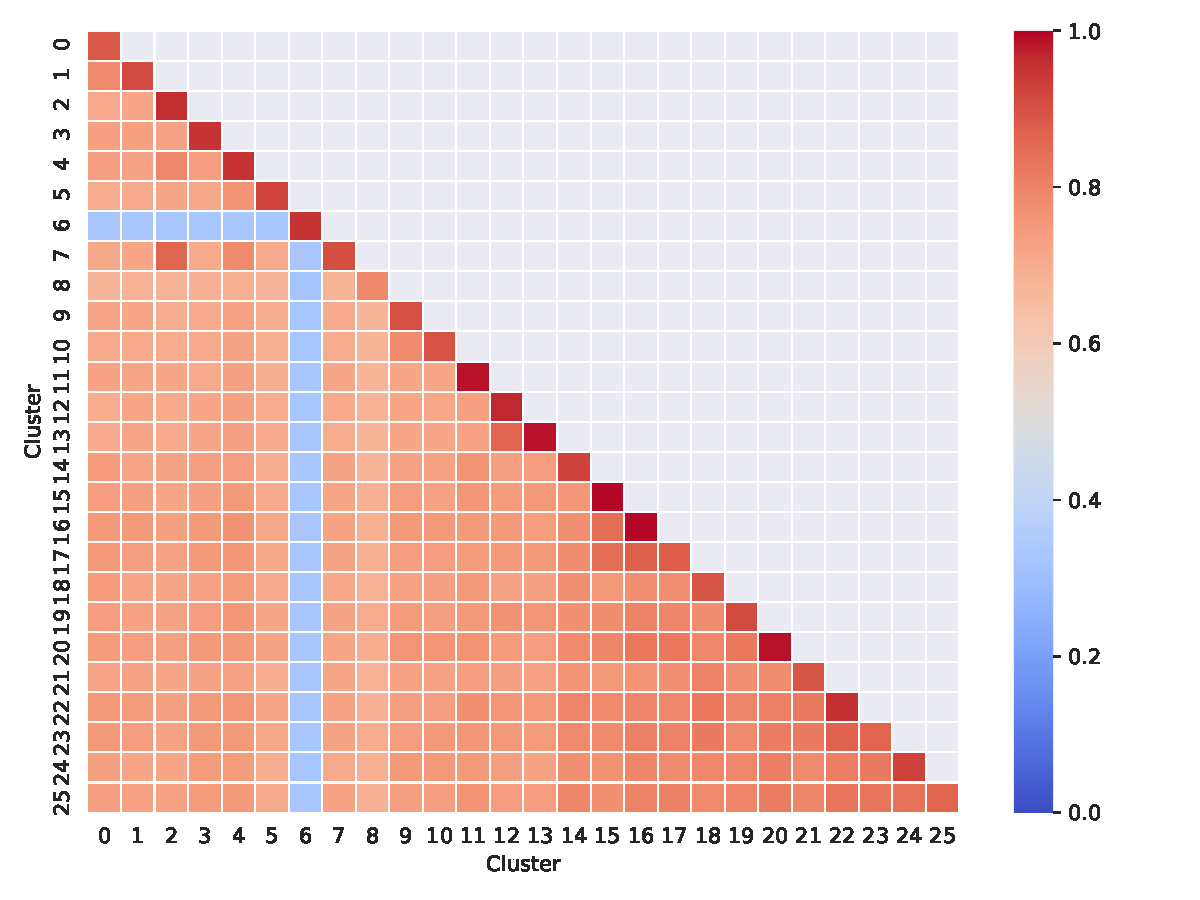
\includegraphics[width=\textwidth]{Results/Cluster_Difference_Segment_5.pdf}
%     \caption[Similarity matrix of segment 5 clusters]{\textbf{Similarity matrix of segment 5 clusters.} }
%     \label{fig:Proof_Clustertree_Segment_5}
% \end{figure}

% \newpage

% \begin{figure}[!hbt]
%     \centering
%     \begin{subfigure}[b]{0.475\textwidth}
%         \caption[Kneedle Algorithm]{\textbf{Kneedle Algorithm}}
%         \label{subfig:Result_Cluster_Knee_Kneedle_6}            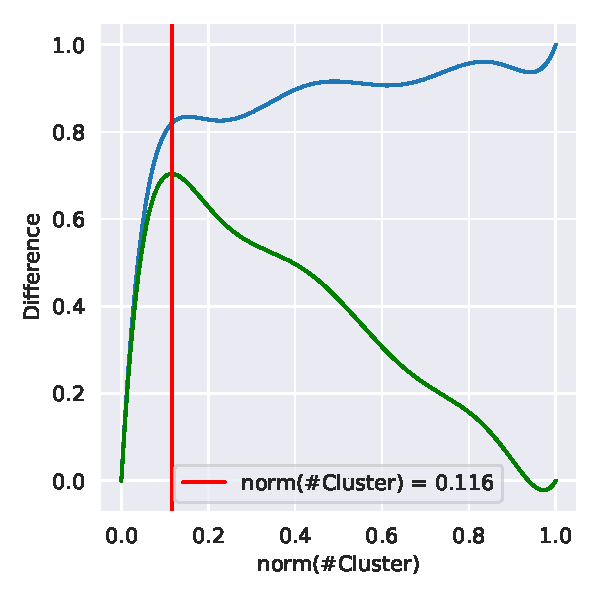
\includegraphics[width=\textwidth]{Results/Cluster_Knee_Segment_6.pdf}
%     \end{subfigure}
%     \hfill
%     \begin{subfigure}[b]{0.475\textwidth}
%         \caption[Kneedle point]{\textbf{Knee point}}
%         \label{subfig:Result_Cluster_Knee_Elbow_6}            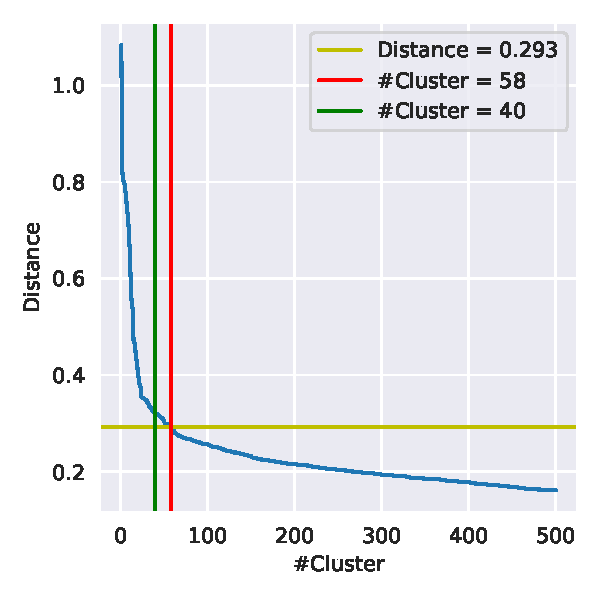
\includegraphics[width=\textwidth]{Results/Cluster_Elbow_Knee_Segment_6.pdf}
%     \end{subfigure}
%     \vskip\baselineskip
%     \begin{subfigure}[b]{0.475\textwidth}
%         \caption[Cluster distribution]{\textbf{Cluster distribution}}
%         \label{subfig:Result_Cluster_Knee_Distributione_6}            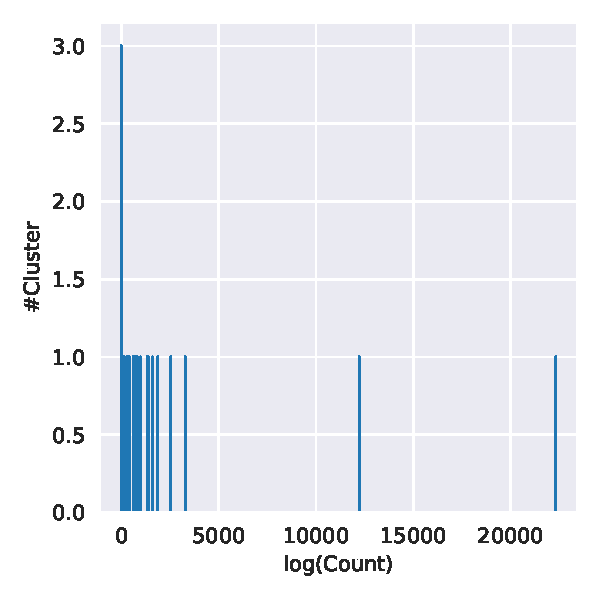
\includegraphics[width=\textwidth]{Results/Cluster_Distribution_Segment_6.pdf}
%     \end{subfigure}
%     \hfill
%     \begin{subfigure}[b]{0.475\textwidth}
%         \caption[Logarithmic distribution]{\textbf{Logarithmic distribution}}
%         \label{subfig:Result_Cluster_Knee_Distribution_log_6}            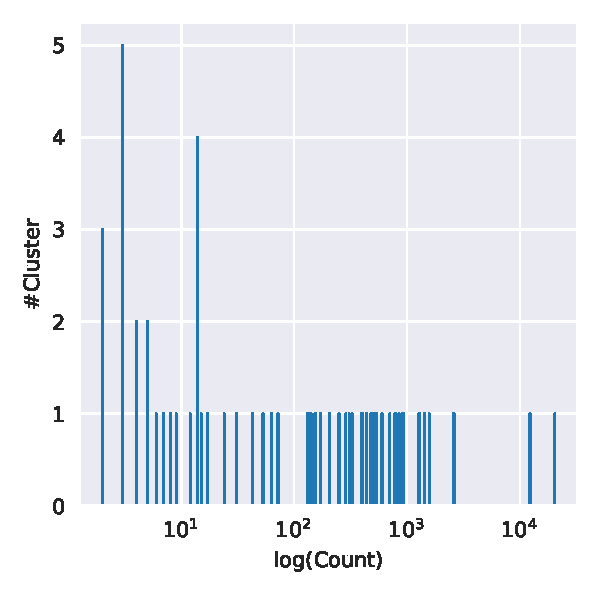
\includegraphics[width=\textwidth]{Results/Cluster_Distribution_Log_Segment_6.pdf}
%     \end{subfigure}
%     \caption[Clustering of segment 6]{\textbf{Clustering of segment 6.} }
%     \label{fig:Result_Cluster_Knee_6}
% \end{figure}

% \newpage

% \begin{figure}[!hbt]
%     \centering
%     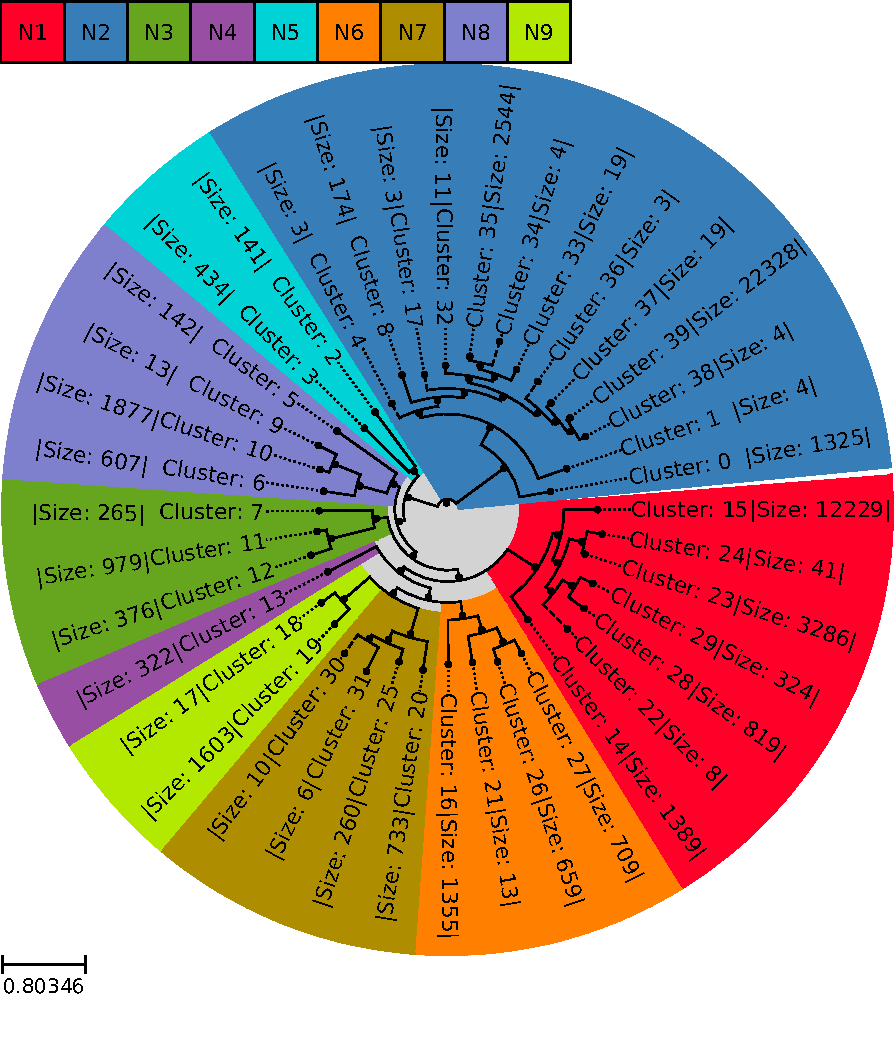
\includegraphics[width=\textwidth]{Results/Clustertree_Segment_6.pdf}
%     \caption[Clustering tree of segment 6]{\textbf{Clustering tree of segment 6.} }
%     \label{fig:Result_Clustertree_Segment_6}
% \end{figure}

% \newpage

% \begin{figure}[!hbt]
%     \centering
%     \includegraphics[width=\textwidth]{Results/Cluster_Difference_Segment_6.pdf}
%     \caption[Similarity matrix of segment 6 clusters]{\textbf{Similarity matrix of segment 6 clusters.} }
%     \label{fig:Proof_Clustertree_Segment_6}
% \end{figure}

% \newpage

% \begin{figure}[!hbt]
%     \centering
%     \begin{subfigure}[b]{0.475\textwidth}
%         \caption[Kneedle Algorithm]{\textbf{Kneedle Algorithm}}
%         \label{subfig:Result_Cluster_Knee_Kneedle_7}            \includegraphics[width=\textwidth]{Results/Cluster_Knee_Segment_7.pdf}
%     \end{subfigure}
%     \hfill
%     \begin{subfigure}[b]{0.475\textwidth}
%         \caption[Kneedle point]{\textbf{Knee point}}
%         \label{subfig:Result_Cluster_Knee_Elbow_7}            \includegraphics[width=\textwidth]{Results/Cluster_Elbow_Knee_Segment_7.pdf}
%     \end{subfigure}
%     \vskip\baselineskip
%     \begin{subfigure}[b]{0.475\textwidth}
%         \caption[Cluster distribution]{\textbf{Cluster distribution}}
%         \label{subfig:Result_Cluster_Knee_Distributione_7}            \includegraphics[width=\textwidth]{Results/Cluster_Distribution_Segment_7.pdf}
%     \end{subfigure}
%     \hfill
%     \begin{subfigure}[b]{0.475\textwidth}
%         \caption[Logarithmic distribution]{\textbf{Logarithmic distribution}}
%         \label{subfig:Result_Cluster_Knee_Distribution_log_7}            \includegraphics[width=\textwidth]{Results/Cluster_Distribution_Log_Segment_7.pdf}
%     \end{subfigure}
%     \caption[Clustering of segment 7]{\textbf{Clustering of segment 7.} }
%     \label{fig:Result_Cluster_Knee_7}
% \end{figure}

% \newpage

% \begin{figure}[!hbt]
%     \centering
%     \includegraphics[width=\textwidth]{Results/Clustertree_Segment_7.pdf}
%     \caption[Clustering tree of segment 7]{\textbf{Clustering tree of segment 7.} }
%     \label{fig:Result_Clustertree_Segment_7}
% \end{figure}

% \newpage

% \begin{figure}[!hbt]
%     \centering
%     \includegraphics[width=\textwidth]{Results/Cluster_Difference_Segment_7.pdf}
%     \caption[Similarity matrix of segment 7 clusters]{\textbf{Similarity matrix of segment 7 clusters.} }
%     \label{fig:Proof_Clustertree_Segment_7}
% \end{figure}

% \newpage

% \begin{figure}[!hbt]
%     \centering
%     \begin{subfigure}[b]{0.475\textwidth}
%         \caption[Kneedle Algorithm]{\textbf{Kneedle Algorithm}}
%         \label{subfig:Result_Cluster_Knee_Kneedle_8}            \includegraphics[width=\textwidth]{Results/Cluster_Knee_Segment_8.pdf}
%     \end{subfigure}
%     \hfill
%     \begin{subfigure}[b]{0.475\textwidth}
%         \caption[Kneedle point]{\textbf{Knee point}}
%         \label{subfig:Result_Cluster_Knee_Elbow_8}            \includegraphics[width=\textwidth]{Results/Cluster_Elbow_Knee_Segment_8.pdf}
%     \end{subfigure}
%     \vskip\baselineskip
%     \begin{subfigure}[b]{0.475\textwidth}
%         \caption[Cluster distribution]{\textbf{Cluster distribution}}
%         \label{subfig:Result_Cluster_Knee_Distributione_8}            \includegraphics[width=\textwidth]{Results/Cluster_Distribution_Segment_8.pdf}
%     \end{subfigure}
%     \hfill
%     \begin{subfigure}[b]{0.475\textwidth}
%         \caption[Logarithmic distribution]{\textbf{Logarithmic distribution}}
%         \label{subfig:Result_Cluster_Knee_Distribution_log_8}            \includegraphics[width=\textwidth]{Results/Cluster_Distribution_Log_Segment_8.pdf}
%     \end{subfigure}
%     \caption[Clustering of segment 8]{\textbf{Clustering of segment 8.} }
%     \label{fig:Result_Cluster_Knee_8}
% \end{figure}

% \newpage

% \begin{figure}[!hbt]
%     \centering
%     \includegraphics[width=\textwidth]{Results/Clustertree_Segment_8.pdf}
%     \caption[Clustering tree of segment 8]{\textbf{Clustering tree of segment 8.} }
%     \label{fig:Result_Clustertree_Segment_8}
% \end{figure}

% \newpage

% \begin{figure}[!hbt]
%     \centering
%     \includegraphics[width=\textwidth]{Results/Cluster_Difference_Segment_8.pdf}
%     \caption[Similarity matrix of segment 8 clusters]{\textbf{Similarity matrix of segment 8 clusters.} }
%     \label{fig:Proof_Clustertree_Segment_8}
% \end{figure}